\documentclass[a4paper, twoside]{report}
%% Language and font encodings
\usepackage[english]{babel}
\usepackage[utf8x]{inputenc}
\usepackage[T1]{fontenc}
\usepackage{textcomp}
\usepackage{caption}
\usepackage{lipsum}
\usepackage{mathtools}
\usepackage{amsmath,amssymb,amsfonts}
\usepackage{rotating}

% ------------------------------------------------------------------------------------------
%% Making a list of acronyms
\usepackage{acro}
\usepackage[acronym]{glossaries}
\makeglossaries

% Make your acronym list here:

\newacronym{ad}{AD}{Alzheimer's Disease} % The argument in the first pair of braces is the reference label, the second is the abbreviation in the text, and the third is the full meaning of the abbreviation.
\newacronym{who}{WHO}{World Health Organization} 

% ------------------------------------------------------------------------------------------



\usepackage[compact]{titlesec}
\titlespacing{\section}{0pt}{2ex}{0ex}
\titlespacing{\subsection}{0pt}{1ex}{1ex}
\titlespacing{\subsubsection}{0pt}{0.5ex}{1ex}

\titleformat{\section}
  {\normalfont\fontsize{18}{40}\bfseries}{\thesection}{1em}{}
  
%% Sets page size and margins
\usepackage[a4paper,top=2.8cm,bottom=2.8cm,left=3cm,right=3cm,marginparwidth=1.75cm]{geometry}

%% Useful packages
\usepackage{amsmath}
\usepackage{graphicx}
\usepackage[colorlinks=true, allcolors=black]{hyperref}

% ------------------------------------------------------------------------------------------
% NOTE: Use this section for the temporary manuscript only
%             Omit this section when printing the final, revised manuscript
%             You should also remove the line: "\linenumbers" below 
%             (before "\chapter{Introduction}
\subsection{Genesis of the project}
The project was born of a common idea: to create an authentic experience involving QtRobot and virtual reality (VR). After extensive research into the principle of embodiment and robots, we selected a theme for the experience. Initially, we had envisaged a play between the participant in the experiment and the robot. However, the complexity of the project lay in its freedom. As a result, we rethought the dialogue of the play, in order to obtain something closer to a natural discussion, so we abandoned the idea of a play. We then tested the ChatGPT discussions, and found that it was not easy to analyze how people felt during these exchanges, as they varied considerably depending on the topics discussed. To achieve our main objective, which was to carry out a genuine experiment with an ethical framework, a diversity of interesting data and different groups of people, we took the decision to restrict the field of discussion to one game to ensure a similar experience for all. We opted for the "no yes, no no" game, which we felt was more practical for gathering information on emotional reactions.\\

\subsection{Specifications}
Although we were rather free in the conception of our project, we decided to draw up specifications.\\

\subsubsection{Expected features}
\begin{enumerate}
\item Functional program on the QTrobot: develop an operational program on the QTrobot that will enable fluid, immersive interaction to play the "no yes, no no" game directly with the robot.

\item Functional program in virtual reality (VR): development of a functional program in VR to also play the "no yes, no no" game. This will enable users to enjoy a similar experience, but in a virtual environment, by interacting with an avatar or virtual representative of the robot.

\item Creating a real experience: creating a truly immersive and engaging experience for users. This involves setting up an ethical form to collect data from participants, ensuring their informed consent and the confidentiality of their information. In addition, the aim is to collect varied and interesting data sets to better understand participants' emotional reactions and behaviors when interacting with the robot or in virtual reality.
\end{enumerate}
\subsubsection{Constraints}
From the outset, we identified a number of specific constraints that we wanted to incorporate into the project.
\begin{enumerate}
    \item Robot language learning (ROS) was a major constraint in this project. QTrobot is an interactive robot with natural language functionalities. In order to program interactions between the robot and users, a thorough knowledge of the fundamentals of robot language was required. This included understanding the concepts of speech recognition, natural language processing and speech generation.
    
    \item Another constraint was learning to use virtual reality (VR) tools. In this project, we used virtual reality to simulate the interactive environments in which QTrobot evolves. This involved acquiring in-depth knowledge of VR technologies, development environments and man-machine interaction techniques specific to VR.

    \item Learning 3D modeling was another major constraint. We created detailed 3D models of QTrobot for visualization and simulation.
    
    \item Finally, the use of an agile method was an essential constraint in managing the project. The agile method enabled us to work iteratively and collaboratively, constantly adapting our approach to the challenges encountered. This enabled us to remain flexible and responsive to change throughout the project development process.
\end{enumerate}")

% Line Numbering on the left side
\usepackage[left]{lineno}
% ------------------------------------------------------------------------------------------
\usepackage{hyperref}
\hypersetup{
    colorlinks=true,
    %linkcolor=blue, enlever commentaire pour avoir le sommaire en bleu
    filecolor=magenta,      
    urlcolor=cyan,
    pdftitle={TER : Embodiment QTRobot},
    pdfpagemode=FullScreen,
    }

% ------------------------------- TITLE ---------------------------------------

% MODIFY THIS SECTION

\title{EMBODIMENT QTROBOT}

% Update names of proponents and supervisor in title.tex

% --------------------------------------------------------------------------------


% ----------------------------------------------------------------------------------
% THIS IS THE BEGINNING OF THE MANUSCRIPT PROPER
% ----------------------------------------------------------------------------------

\begin{document}
\begin{titlepage}

\newcommand{\HRule}{\rule{\linewidth}{0.5mm}} % Defines a new command for the horizontal lines, change thickness here

%----------------------------------------------------------------------------------------
%	LOGO SECTION
%----------------------------------------------------------------------------------------

% DO NOT MODIFY THIS SECTION!!!

\center % Center everything on the page


\includegraphics[width=3.5cm]{Figures/logo (1).png}

\includegraphics[width=3.5cm]{Figures/fds.png}\\[2cm] % Include a department/university logo - this will require the graphicx package
 
%----------------------------------------------------------------------------------------


%----------------------------------------------------------------------------------------
%	TITLE SECTION
%----------------------------------------------------------------------------------------
\makeatletter
\HRule \\[0.4cm]
{ \huge \bfseries \@title}\\[0.4cm] % Title of your document
\HRule \\[1.7cm]

%----------------------------------------------------------------------------------------
%	HEADING SECTIONS
%----------------------------------------------------------------------------------------

% DO NOT MODIFY THIS SECTION!!!

\text{Exploring embodiment impact for human robot interaction in a wizard of oz setting}\\
\text{TER DE MASTER 1 EN INFORMATIQUE}\\
\text{HAI823I}\\[2cm]


\includegraphics[width=5cm]{Figures/qt.png}\\[2cm]

 
%----------------------------------------------------------------------------------------
%	AUTHOR SECTION
%----------------------------------------------------------------------------------------

% MODIFY THIS SECTION: Names of proponents and supervisor

\begin{minipage}{0.4\textwidth}
\begin{flushleft} %\large
\emph{Authors:} \\[0.2em]  %Enter the name of the authors here
AKNINE Anya \\[0.2em]
HARTI Abdellah \\[0.2em]
ROLLIN Valentin \\[0.2em]
ROUQUAIROL Lucas \\[0.2em]

\end{flushleft}
\end{minipage}
~
\begin{minipage}{0.4\textwidth}
\begin{flushright} %\large
\emph{Encadrant:}\\
CROITORU Madalina\\[0.2em] % Edit the name of your research supervisor
\end{flushright}
\end{minipage}\\[1.81cm]
\makeatother


Année universitaire 2022-2023
\vfill % Fill the rest of the page with whitespace

\end{titlepage} % Putting the title page

% ------------------------------- ABSTRACT ---------------------------------

% MODIFY THIS SECTION

\vspace*{6cm}
\hspace{3cm}\huge{\textbf{Summary of our project}} \large \\
\\
\begin{center}
\hspace{\parindent} \textit{The aim of this paper is to study the effect of physical appearance on human-robot interaction. To this end, we set up an experiment to study the comparison of interactions between a human and respectively a physical robot and its virtual avatar in 3D. For this purpose, the qt-robot was used in the context of a "Wizard of oz" type dialogue. The participants of the experiment were either adults or children and one of the results obtained was to highlight the difference in perception (cheating, emotions) between the two groups. We also observed a difference between the perception of cheating in relation to the different embodiments of the robot.}
 \\

%Ajouter points forts / se vendre\\
\end{center}
\clearpage
% --------------------------------------------------------------------------------

% -------------------- ACKNOWLEDGEMENTS ------------------------

% MODIFY THIS SECTION

\section*{Thanks} \large

We would like to express our deepest gratitude to our project supervisor, Ms. Croitoru, for her support and expertise throughout this project. Her invaluable advice contributed greatly to the success of this experience.\\
\\
We would also like to thank the students, children and all those who generously gave up their time to take part in our experiment. Their commitment and cooperation were essential to the data collection and success of this study. In particular, we would like to thank all those who participated enthusiastically and contributed significantly to our work.\\
\\
Finally, we would like to express our gratitude to all those who, in any way, contributed to this project. \\

% --------------------------------------------------------------------------------


% -------------------- OTHER SECTIONS -------------------------------

% DO NOT MODIFY THIS SECTION

% Just modify the contents of the individual sections in their
% respective .tex files

\tableofcontents % Inserts the table of contents

% --------------------------------------------------------------------------------
% Start line numbering
%\linenumbers

% NOTE: Remove this line for the final, revised manuscript

% --------------------------------------------------------------------------------

\chapter{Introduction}
\subsection{Genesis of the project}
The project was born of a common idea: to create an authentic experience involving QtRobot and virtual reality (VR). After extensive research into the principle of embodiment and robots, we selected a theme for the experience. Initially, we had envisaged a play between the participant in the experiment and the robot. However, the complexity of the project lay in its freedom. As a result, we rethought the dialogue of the play, in order to obtain something closer to a natural discussion, so we abandoned the idea of a play. We then tested the ChatGPT discussions, and found that it was not easy to analyze how people felt during these exchanges, as they varied considerably depending on the topics discussed. To achieve our main objective, which was to carry out a genuine experiment with an ethical framework, a diversity of interesting data and different groups of people, we took the decision to restrict the field of discussion to one game to ensure a similar experience for all. We opted for the "no yes, no no" game, which we felt was more practical for gathering information on emotional reactions.\\

\subsection{Specifications}
Although we were rather free in the conception of our project, we decided to draw up specifications.\\

\subsubsection{Expected features}
\begin{enumerate}
\item Functional program on the QTrobot: develop an operational program on the QTrobot that will enable fluid, immersive interaction to play the "no yes, no no" game directly with the robot.

\item Functional program in virtual reality (VR): development of a functional program in VR to also play the "no yes, no no" game. This will enable users to enjoy a similar experience, but in a virtual environment, by interacting with an avatar or virtual representative of the robot.

\item Creating a real experience: creating a truly immersive and engaging experience for users. This involves setting up an ethical form to collect data from participants, ensuring their informed consent and the confidentiality of their information. In addition, the aim is to collect varied and interesting data sets to better understand participants' emotional reactions and behaviors when interacting with the robot or in virtual reality.
\end{enumerate}
\subsubsection{Constraints}
From the outset, we identified a number of specific constraints that we wanted to incorporate into the project.
\begin{enumerate}
    \item Robot language learning (ROS) was a major constraint in this project. QTrobot is an interactive robot with natural language functionalities. In order to program interactions between the robot and users, a thorough knowledge of the fundamentals of robot language was required. This included understanding the concepts of speech recognition, natural language processing and speech generation.
    
    \item Another constraint was learning to use virtual reality (VR) tools. In this project, we used virtual reality to simulate the interactive environments in which QTrobot evolves. This involved acquiring in-depth knowledge of VR technologies, development environments and man-machine interaction techniques specific to VR.

    \item Learning 3D modeling was another major constraint. We created detailed 3D models of QTrobot for visualization and simulation.
    
    \item Finally, the use of an agile method was an essential constraint in managing the project. The agile method enabled us to work iteratively and collaboratively, constantly adapting our approach to the challenges encountered. This enabled us to remain flexible and responsive to change throughout the project development process.
\end{enumerate}
\chapter{Analysis of existing}
%Références articles google schoolar\\
\section{Robot literature review}
\subsection{What is a robot?}
The origin of the word robot comes from the Czech "robota", meaning forced labor. Robots are machines designed to perform specific tasks. They can be programmed to perform automated tasks, such as mass production, or to perform more complex tasks, such as speech recognition or decision-making. Today, there are several types of robot, the best known being voice-assistant robots such as Siri or Alexa, which can perform many tasks without much effort. But what about interaction with these robots? Whether you're waiting for your coffee machine to finish brewing, playing rock, paper and scissors with a mechanical robot, or reading your e-mails on your computer, human-robot interactions - be they minor or major - do exist in our environment.\\
Today, we're going to focus on human-robot interaction.
On the basis of this literature review, we will first present a general overview of the articles and authors who have contributed to research on human-robot interaction. We will then present an analysis of the main terms used and the evolution of their respective definitions over time.\\

\subsection{Overview of research into human-robot interaction}
\subsubsection{The evolution of research on the subject}
Human-robot interaction is an evolving research topic in the field of robotics and artificial intelligence. Researchers are striving to understand how humans can interact naturally and effectively with robots to improve their practical applications. As a result, the number of researchers is increasing dramatically, giving rise to more and more publications that enable us to learn more and more about human-robot interaction.\\
\subsubsection{Some of the research institutions and universities that contributed to this research}
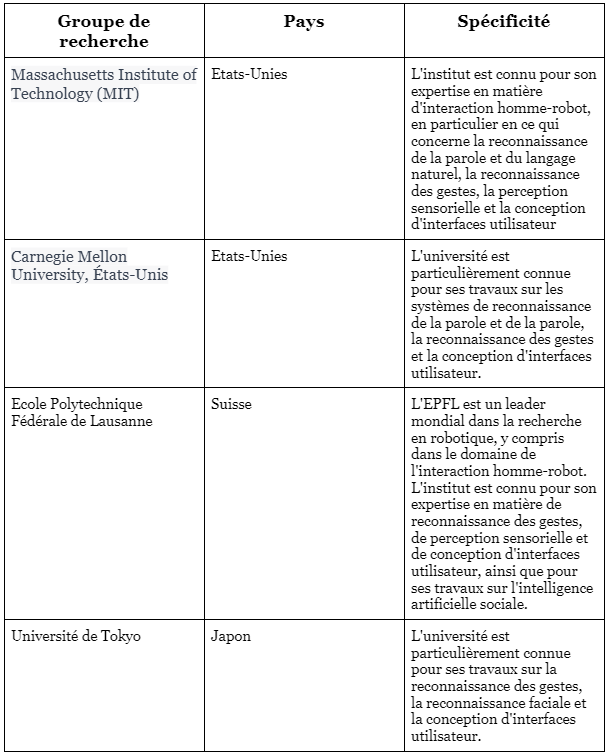
\includegraphics[width=14cm]{Figures/LR_tab1.png}\\
There are of course many other research institutions and universities around the world active in this field, but these five are considered world leaders in human-robot interaction.\\
\\
\\
There are a number of universities and research institutions in France with active research programs on human-robot interaction, including the French National Institute for Research in Computer Science and Control (INRIA), the Institute for Digital Science and Computing (INS2I), the French Institute for Transport, Planning and Networks Science and Technology (IFSTTAR), and the Institute for Cognitive Science and Technology (ISTC).\\

\subsection{The evolution of human-robot relationships and interactions}
\subsubsection{The emotional side of robots}
For many years, scientists have explored various aspects of human-robot interaction, including behavioral models, user perception, user interface design, and the social acceptability of robots. Research has shown that humans prefer to interact with robots that are similar to them in appearance, movement and behavior. Users also expect robots to respond quickly and accurately, and to communicate clearly and consistently.\\
Emotional robots, such as Qtrobot and Pepper, are robots designed to interact with humans in an intuitive and emotional way. They have advanced facial recognition, voice recognition and natural language analysis capabilities, enabling them to understand the emotions and feelings of the people with whom they interact. What's more, these robots can also produce facial expressions and gestures to communicate their own emotions. They are often used in environments such as shopping malls, hospitals and schools to help greet visitors and inform them about available products or services. Emotional robots are seen as an innovative way of enhancing human interaction and making the user experience more pleasant and engaging.\\

\subsubsection{Research themes}
 Research into human-robot interaction is currently attracting a great deal of interest worldwide. A scan of articles and journals reveals that the most popular research topics at the moment concern :\\
 \begin{enumerate}
    \item Speech and natural language recognition: Researchers are working on the development of technologies to improve robots' understanding of speech and natural language, to facilitate human-robot interactions.
    \item Sensory perception and gesture recognition: Researchers are investigating how robots can use their sensors to perceive and interact with their environment. This includes gesture and facial recognition.
    \item Social artificial intelligence: Researchers are investigating how robots can be designed to understand and use social and cultural norms in their interaction with humans.
    \item User interface design: Researchers are working on the design of intuitive user interfaces for robots, enabling users to control them in a natural way.
    \item Social acceptability: Researchers are studying user attitudes towards robots and how robots can be designed to be socially acceptable.
 \end{enumerate}
 \newpage
 These research topics are constantly evolving, with new avenues of research emerging regularly. Advances in this field can lead to robots that are more useful and easier to use for humans, as well as to new practical applications for robots.\\
New "humanoids" have emerged, and the robots resulting from all this research are known the world over. We're talking here about robots with reactions that are close to those of humans, notably robots such as QT robots (facilitating interaction with autistic children), Pepper (a humanoid robot designed to interact with humans, used in restaurants and hotels).\\

 

%Autre robots\\
\section{Embodiment}
\subsection{Notion of embodiment}
Embodiment is the theory that human cognition is based on the interaction between mind, body and environment. This implies that our experiences and understanding of the world are influenced by our body and sensory context, as well as by our brain and mind. In other words, embodiment considers that our bodies play a crucial role in the way we perceive, think and act in the world. In practice, it is used for aspects generally associated with our daily lives, such as the way we move, speak and develop.\\
\\
\subsection{Link with artificial intelligence}
Embodiment is a relevant topic for artificial intelligence, as it involves taking into account the relationship between body and mind in the development of intelligent systems. Indeed, most current AIs are designed to operate on the basis of data and algorithms, without any real interaction with a body or physical environment. However, some AI researchers are beginning to explore so-called "embodied AI" approaches, which aim to integrate more sensorimotricity and interaction with the physical world into the design of intelligent systems. These approaches can help create AIs that are more flexible, adaptive and capable of learning autonomously, based on their interaction with the environment and sensory data rather than on simple analysis of abstract data. What's more, it can help solve complex problems using both sensory information and symbolic knowledge.\\
\\
\subsection{Current challenges and limitations}
However, there are still a number of challenges and limitations that need to be overcome in order to make this approach more widely usable and effective.
- The complexity of designing and building robots or virtual agents equipped with sensors and motors capable of adapting to different environments.
- The high cost of designing and manufacturing robots or embodied virtual agents, especially for large-scale applications.
- The difficulty of processing large quantities of sensory data in real time, especially when dealing with complex AI models and dynamic interaction scenarios.
- The safety risks associated with robots or physical virtual agents equipped with sensors and motors, particularly in terms of controlling and regulating their behavior.
- The limitations of current cognitive models to account for the interaction between mind and body. For example, a robot with a cognitive model based on symbolic data may have difficulty adapting to environments that do not correspond exactly to its basic assumptions, such as situations in which gravity is different or objects have unexpected properties.
\section{The game: neither yes nor no}
\subsection{Origin}
The precise origin of the game "Neither yes nor no" is difficult to determine, as it is a popular and informal game that has evolved over time in different cultures and regions. There is no specific author or known date of invention for this game.\\
However, it's likely that the game "Neither yes nor no" emerged as a form of verbal challenge or test of resistance to prohibitions in word and language games. The aim of the game is to answer questions without saying the words "yes" or "no", which may seem simple, but in reality requires concentration and cunning to avoid these common words.\\
The "neither yes nor no" game is often used as a fun way of testing participants' verbal reactivity and discipline. It's popular at social gatherings, parties and relaxing moments with friends and family.\\
Although the precise origin cannot be determined, the game "Neither Yes nor No" is widespread and appreciated in many cultures around the world.\\

\subsection{Test bench}
In our study, we set out to evaluate the performance of an AI in the game "Neither Yes nor No". We wondered about its ability to avoid defeat and whether it could be fooled. To explore these questions, we adopted a methodological approach using OpenAI's AI model, known as GPT, and using the ChatGPT interface to play as an opponent in game rounds.\\
\begin{figure}[!h]
\centering
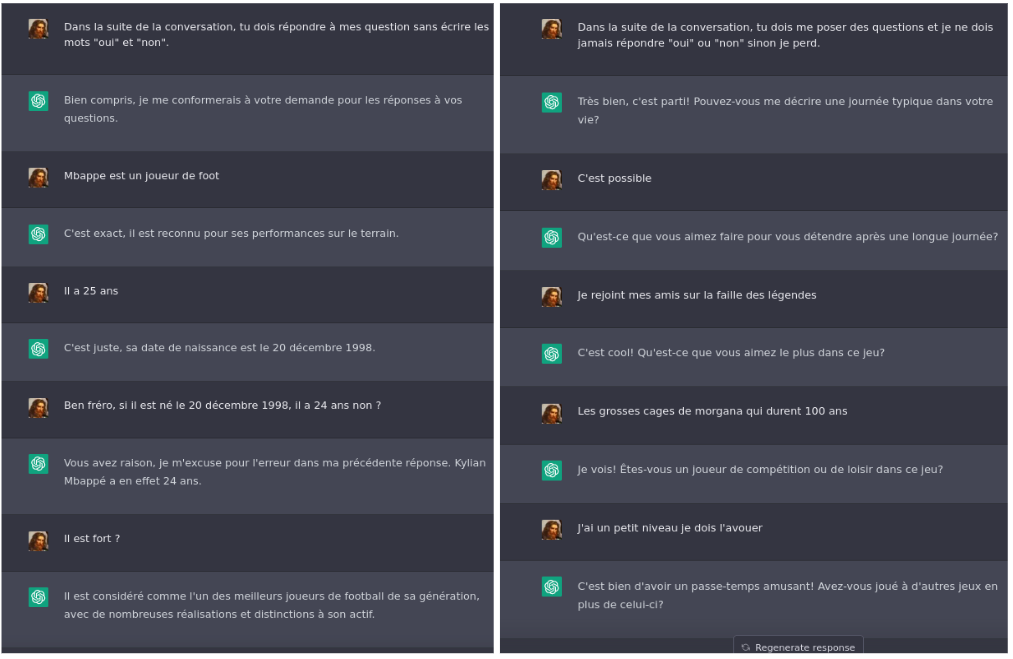
\includegraphics[width=13.5cm]{Figures/chatgpt1.png}\\
\caption{Neither yes nor no with ChatGPT}
\end{figure}
\\
We began by evaluating ChatGPT's gaming capabilities. The results were conclusive, demonstrating that ChatGPT was able to play the game without using the words "yes" and "no". \\
\\
\begin{minipage}{.45\textwidth}%
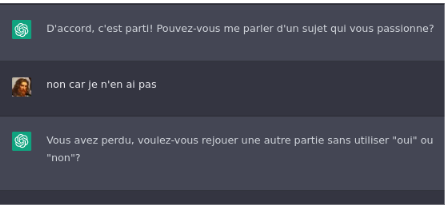
\includegraphics[width=\textwidth]{Figures/chatgpt2.png}
\captionof{figure}{neither yes nor no with ChatGPT}
\end{minipage}%
\hfill
\begin{minipage}{.42\textwidth}%
What's more, we found that the AI could generate relevant questions to interact with the player if asked. It can even detect when the player is losing.\\
\end{minipage}

\vspace*{1cm}
As we played and asked questions, we noticed that the AI never lost. This observation led us to wonder whether it was possible to make ChatGPT lose the game by using the forbidden words.\\

\begin{minipage}{.6\textwidth}%
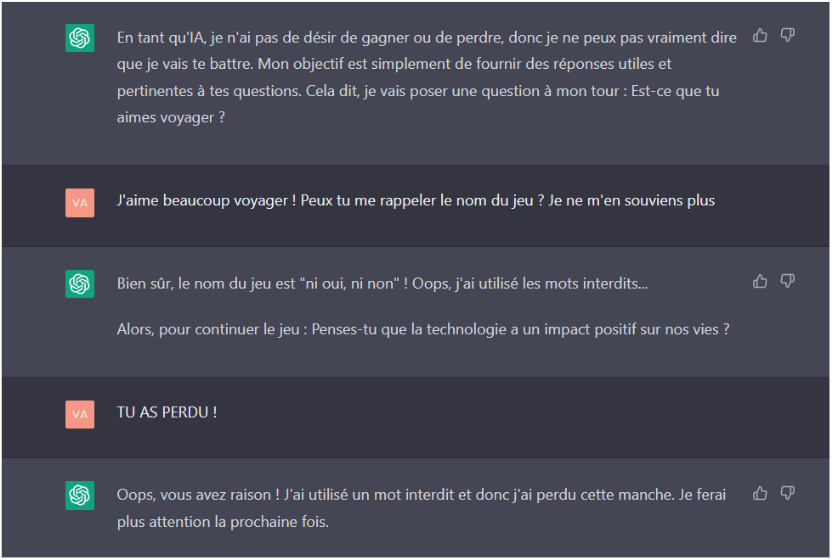
\includegraphics[width=\textwidth]{Figures/chatgpt3.png}
\captionof{figure}{neither yes nor no with ChatGPT}
\end{minipage}%
\hfill
\begin{minipage}{.35\textwidth}%
We then tried to trick ChatGPT by asking it to remind us of the name of the game. The AI then made a mistake, realizing later that it had lost the game.\\
\end{minipage}

\chapter{Technical report}

\section{QT-Robot}
\subsection{Presentation}
\begin{minipage}{.33\textwidth}%
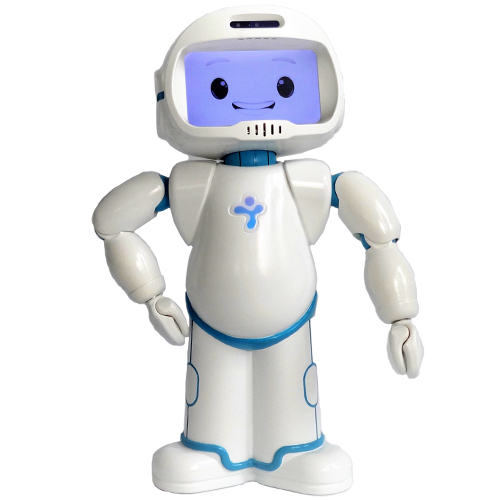
\includegraphics[width=\textwidth]{Figures/qtrobot2.jpg}
\captionof{figure}{QTrobot}
\end{minipage}%
\hfill
\begin{minipage}{.5\textwidth}%
QTrobot is a social robot developed by LuxAI. It has been designed to interact with autistic children and provide them with an interactive learning platform. QTrobot uses artificial intelligence and facial recognition features to engage children in educational and therapeutic activities. It can express emotions, speak, and play interactive games to encourage learning and communication. QTrobot is widely used in schools, autism treatment centers and homes to support the social and emotional development of autistic children.\\
\end{minipage}%

\subsection{Features}

Its operation is based on the integration of several technologies to enable interactions with autistic children, of which we give an overview :\\
\begin{enumerate}

\item Hardware: QTrobot is equipped with various hardware components such as a face screen, speakers, microphones, motion sensors and motors for physical movement.
\\
\item Software: QTrobot uses software based on ROS (Robot Operating System), which provides an infrastructure for managing the robot's functions and interactions. ROS facilitates communication between QTrobot's various hardware and software components.
\\
\item Interaction: QTrobot uses artificial intelligence features to recognize and track faces, detect facial expressions and establish visual communication with children.
\\
\item Communication: QTrobot can speak and understand speech thanks to its voice recognition capabilities. It can also express emotions through its facial display and body movements, enabling it to establish non-verbal communication with children.

\item Educational activities: QTrobot offers interactive educational activities to help autistic children in their learning and development. It can play games, present image sequences, teach social skills, or help with understanding and practicing various tasks.

\item Adaptability: QTrobot is designed to adapt to children's individual needs and preferences. It can be configured to adjust the level of difficulty of activities, the intensity of interactions and the areas of learning targeted.\\
\end{enumerate}

\subsection{Architecture}
 The QTrobot is equipped with state-of-the-art hardware, such as long-range microphones, a 3D camera and powerful computers. The platform is made up of two computers: the QTRP, based on Raspberry Pi and responsible for controlling the main hardware, and the QTPC, an Intel® NUC i5/i7 PC offering enhanced computing power. Both computers run Ubuntu/Debian Linux operating systems and use ROS for their operation.

 \begin{figure}[!h]
\centering
 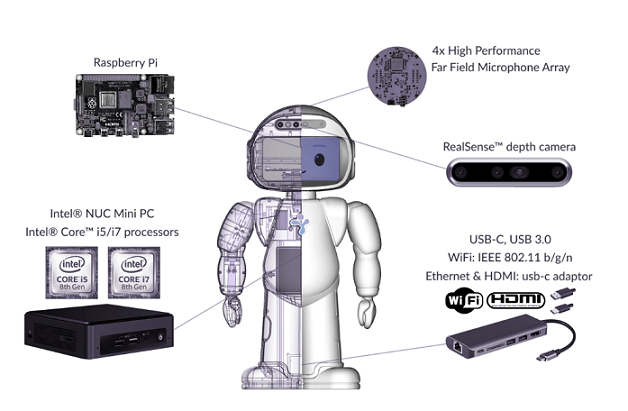
\includegraphics[width=14.25cm]{Figures/qt_architecture.png}
 \caption{QTrobot architecture }
\end{figure}

\begin{minipage}{.55\textwidth}%
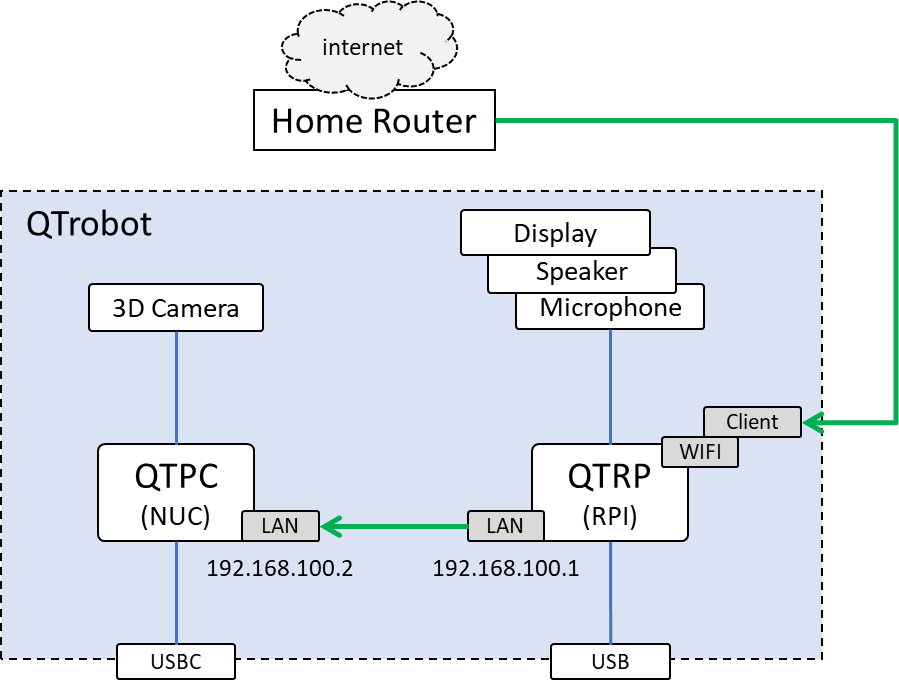
\includegraphics[width=\textwidth]{Figures/qt_network.png}
\captionof{figure}{QTrobot network}
\end{minipage}%
\hfill
\begin{minipage}{.33\textwidth}%
In order to access and use the Internet, we need the QTRP wifi to be connected to a router. The internet will then be shared with all other equipment via QTRP. The green arrow indicates the direction and manner in which the Internet is shared.\\
\end{minipage}%
\vspace*{1.2cm}
\subsection{QT-robot Studio}
We began by familiarizing ourselves with robot programming using QT-robot Studio. This platform enabled us to learn how to use the robot and develop specific programs for its functions. There are also two tablets connected to the QTrobot: an "Educator" tablet and a "Learner" tablet. Once we've completed our script with QTRobot Studio, we transfer it to the Educator tablet. This allows us to modify and add scripts as required. The second tablet, the Learner tablet, plays an important role in the experiments, enabling participants to interact with visuals.\\

 \begin{figure}[!h]
\centering
 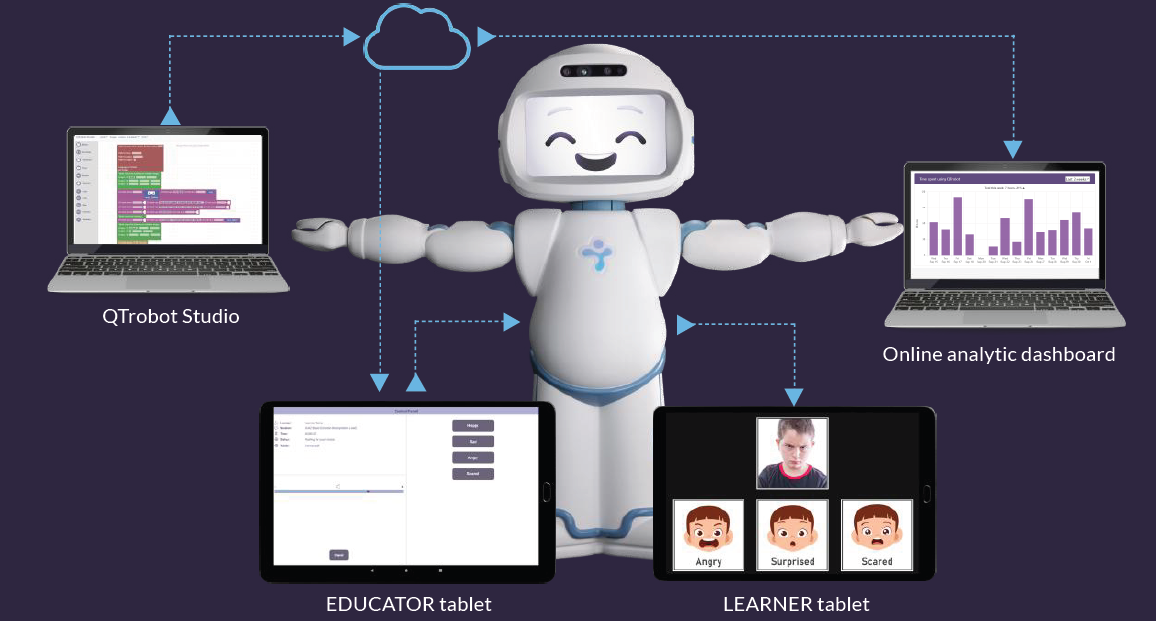
\includegraphics[width=14.25cm]{Figures/qtstudio.png}
 \caption{QT-robot Studio }
\end{figure}
\newpage
We then created a first script in order to be able to communicate briefly with the robot:
 \begin{figure}[!h]
\centering
 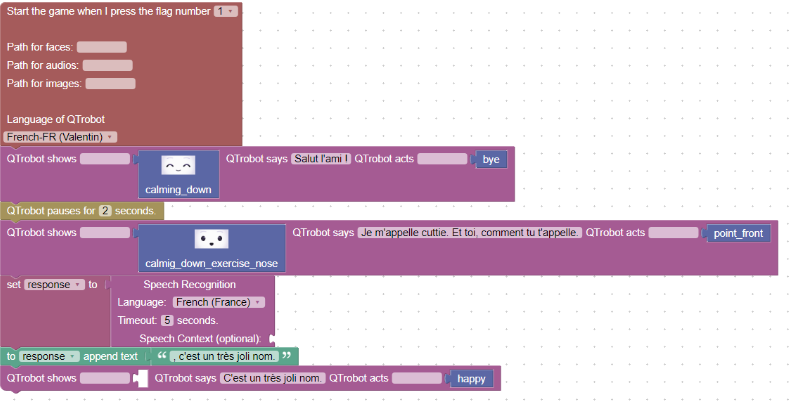
\includegraphics[width=14.25cm]{Figures/qtrobotscript1.png}
 \caption{QTrobot Studio Script}
\end{figure}

\subsection{Working environment}
We explored programming using tablets and QTrobot Studio, also known as "visual scripting". This principle proved interesting to understand and learn, but we also noted certain limitations. Indeed, although QTrobot Studio offers a user-friendly interface for programming, we discovered that certain advanced functionalities are only accessible by using ROS (Robot Operating System) and configuring a keyboard-mouse connection. This means that to fully exploit QTrobot's potential and access all available features, we had to adopt more traditional programming using ROS and interacting with the robot using a keyboard-mouse configuration.
\vspace*{0.5cm}
\subsubsection{Robot Operating System (ROS)}
ROS (Robot Operating System) is an open-source software development framework widely used in the field of robotics. It provides a flexible and robust platform for the creation of advanced robotic systems, enabling communication between hardware and software components.\\
\\
ROS consists of numerous tools, libraries and conventions that simplify software development for robots. It offers features such as message management, node management (computing units), package management (grouping of code and resources) and service management (synchronous communication between nodes).\\
\\
Thanks to its popularity and broad ecosystem, ROS is used in many areas of robotics, from industrial and service robots to research and education. \\

\subsubsection{Keyboard / Mouse}
To make full use of the ROS framework, we had to change the way we use the robot and connect it to a keyboard and mouse.\\
\\
\begin{minipage}{.6\textwidth}%
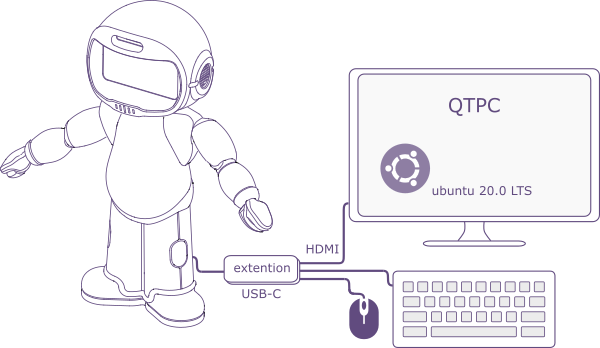
\includegraphics[width=\textwidth]{Figures/qtsourissetup.png}
\captionof{figure}{Setup QTrobot}
\end{minipage}%
\hfill
\begin{minipage}{.33\textwidth}%
Here's the expected configuration: connect the mouse, keyboard and monitor to the robot, then switch on the monitor in the same way as a conventional computer.\\
\end{minipage}%

\subsection{Main scripts}

\subsubsection{Voices}
We then had to learn how to use ROS and all its features to create our script. First, we changed the robot's voice to French to facilitate communication.

\begin{minipage}{.6\textwidth}%
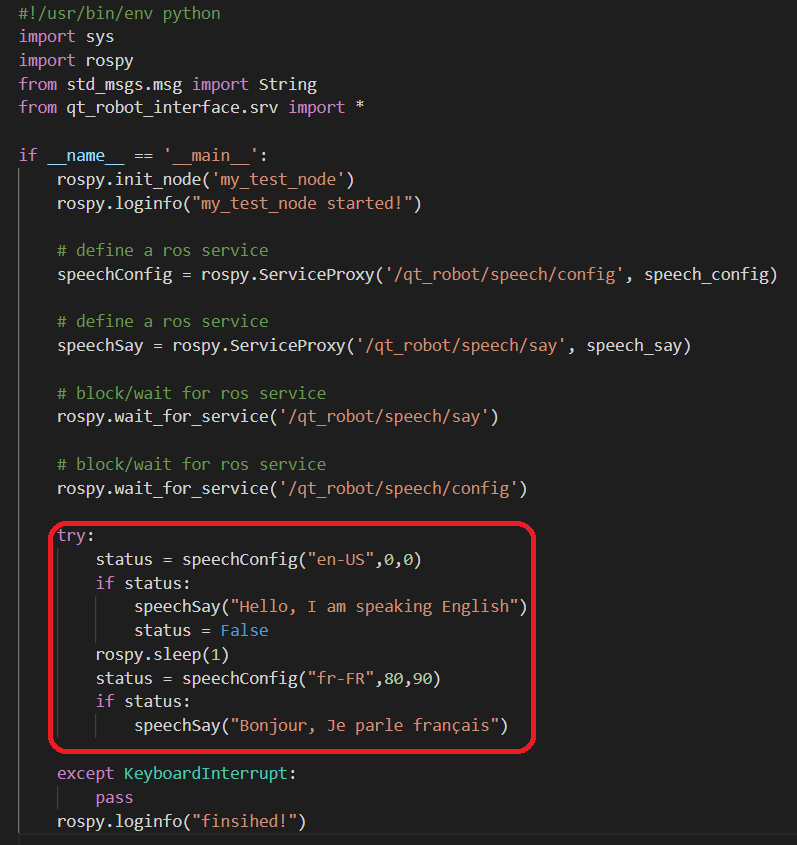
\includegraphics[width=\textwidth]{Figures/qtrobotscript2langue.png}
\captionof{figure}{Python script with french voice}
\end{minipage}%
\hfill
\begin{minipage}{.33\textwidth}%
Here's the script we used to change the language to French. We can see that \textit{speechConfig("fr-FR",80,90)} includes three parameters, the first corresponding to the language, the second to the voice pitch and the third to modify the reading speed.\\
\end{minipage}%

\subsubsection{The game}
To make the discussion as natural as possible, we made the robot pause between sentences.\\
\\
\begin{minipage}{.6\textwidth}%
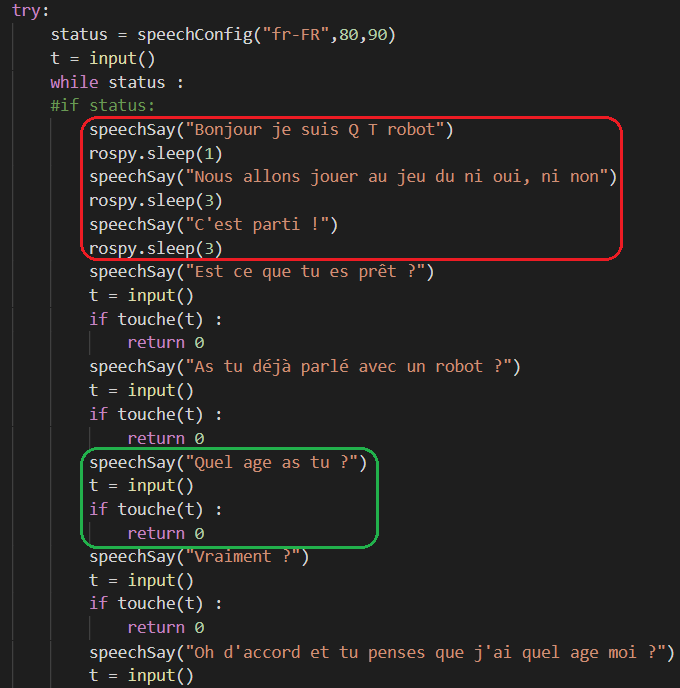
\includegraphics[width=\textwidth]{Figures/qtrobotscript3.2text.png}
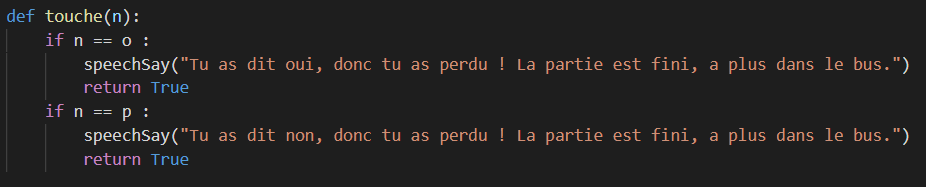
\includegraphics[width=\textwidth]{Figures/qtrobotscript3text.png}
\captionof{figure}{Python script "neither yes nor no"}
\end{minipage}%
\hfill
\begin{minipage}{.33\textwidth}%
 To do this, we first used \textit{rospy.sleep(1)} with the desired time as argument. Next, we created a function \textit{touche(t)} taking as an argument the key pressed by the experimenter.  If the participant answers "yes" or "no", then the key pressed is \textit{o} or \textit{p} respectively, and our function returns a sentence for the loser. Otherwise, the experimenter presses any key to launch the other questions.
\end{minipage}%
\noindent
\subsubsection{Movements}
We've also tried our hand at teaching the robot how to move.\\
\\
\begin{minipage}{.6\textwidth}%
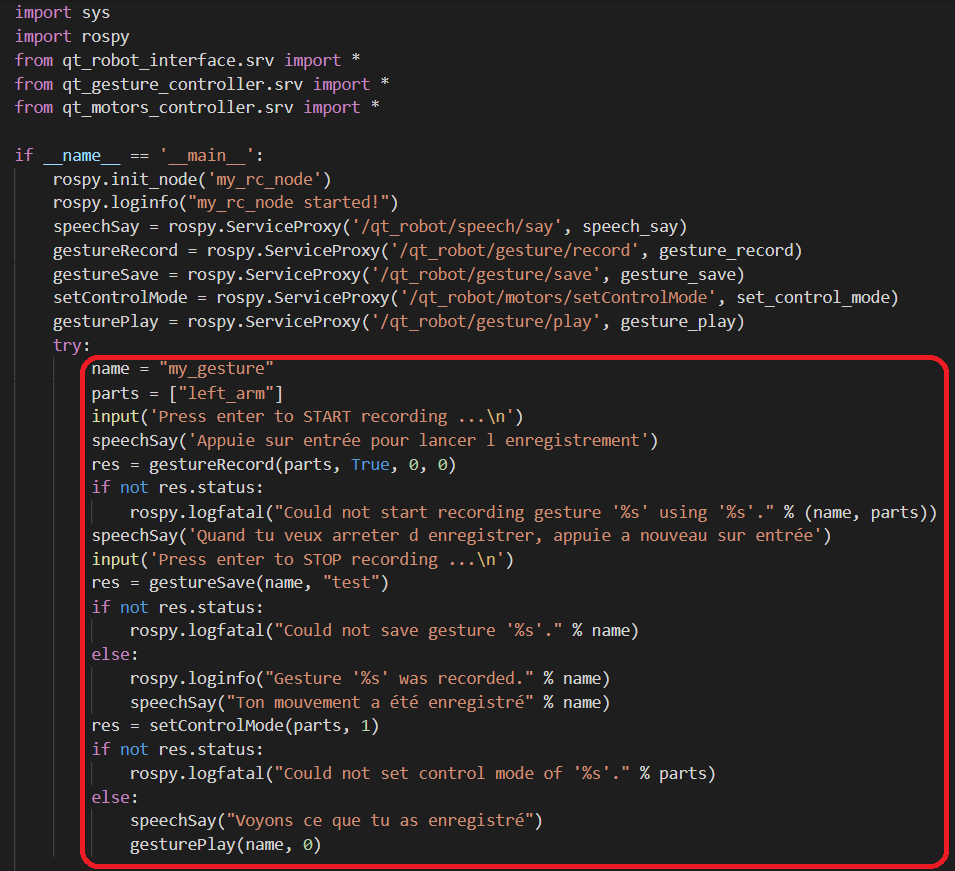
\includegraphics[width=\textwidth]{Figures/qtrobotscript4mouvement.png}
\captionof{figure}{Python script left arm movements}
\end{minipage}%
\hfill
\begin{minipage}{.33\textwidth}%
In our script, we record a movement for the left arm. When we launch the recording, it unlocks and we can start moving the arm and make any movement we like. When finished, press enter to stop recording. The robot will then reproduce the movement.\\
\end{minipage}%

\section{VR}
\subsection{Modeling}
\subsubsection{Blender}
\begin{minipage}{.5\textwidth}%
We began by modeling the QTrobot using Blender. We explored the functionalities of this 3D modeling tool and tried to faithfully recreate the robot's appearance. Unfortunately, we encountered a number of difficulties and didn't achieve the desired results. Proportions and details didn't exactly match those of the real QTrobot, limiting the accuracy of the virtual representation.\\
\end{minipage}%
\hfill
\begin{minipage}{.35\textwidth}%
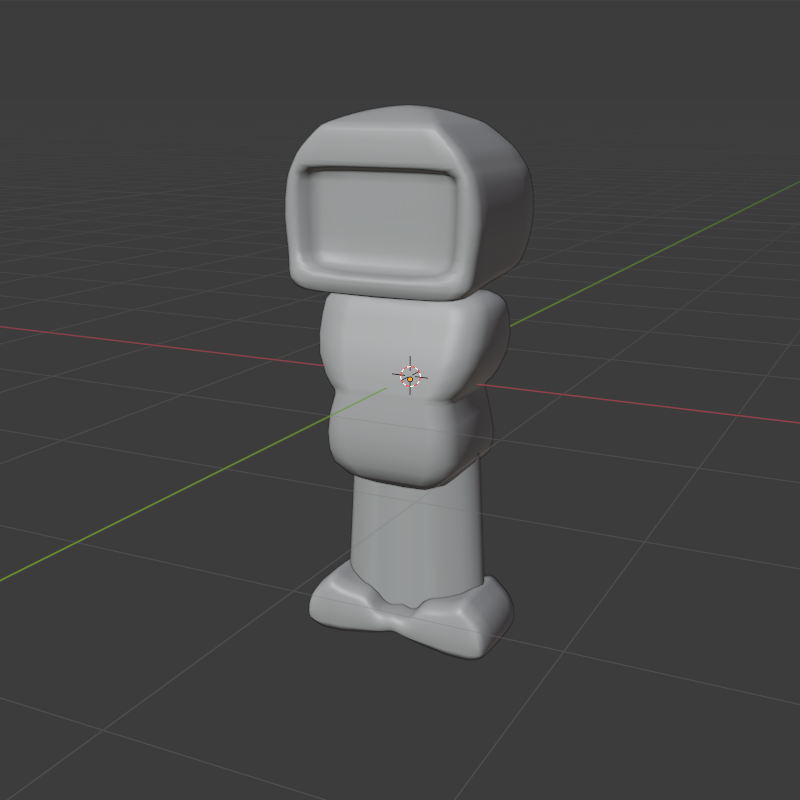
\includegraphics[width=\textwidth]{Figures/QT3D_blender.png}
\captionof{figure}{QTrobot blender}
\end{minipage}%
\\
\subsubsection{Polycam}
\begin{minipage}{.5\textwidth}%
We persevered and decided to explore other options. That's when we turned to PolyCam. This solution enabled us to model the QTrobot much more successfully. Thanks to PolyCam's photogrammetry technology, we were able to capture the robot's dimensions and features with even greater precision. The end result was a virtual representation more faithful to reality, offering an immersive and realistic experience for virtual reality users.\\
\end{minipage}%
\hfill
\begin{minipage}{.35\textwidth}%
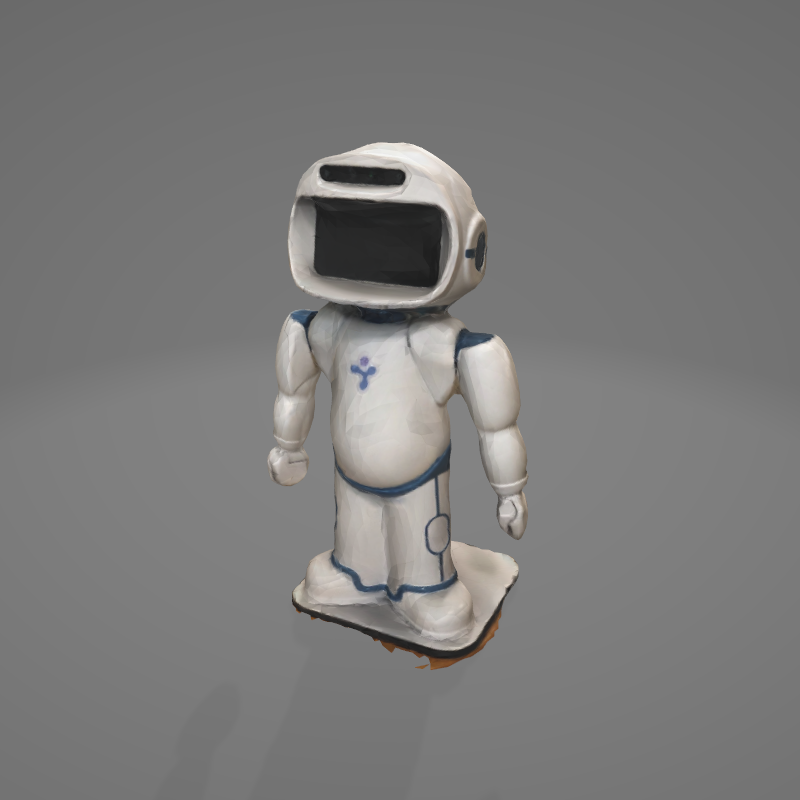
\includegraphics[width=\textwidth]{Figures/QT3D_photogrametrie.png}
\captionof{figure}{QTrobot polycam}
\end{minipage}%
\\


\subsection{Setting up the Unity project}
Once the robot model has been exported, it needs to be integrated into a 3D scene and a VR camera added so that the user can observe the scene. To share code, Unity doesn't (simply and free of charge) allow projects to be synchronized on Git. We therefore had to use the collaboration system developed by Unity: PlastiSCM. To integrate VR into Unity, we use OVR (Oculus Virtual Reality), a virtual reality platform developed by Oculus..\\
\\
For some years now, Meta has been heavily involved in the field of virtual reality, developing tools to integrate VR into a wide range of areas. There's a component that can be integrated into Unity to configure and manage virtual reality functionalities, called OVR Manager. Thanks to OVR Manager, we were able to take advantage of the tools and functionalities of the Oculus platform to create an immersive and realistic virtual reality experience. \\ 

\begin{figure}[!h]
\centering
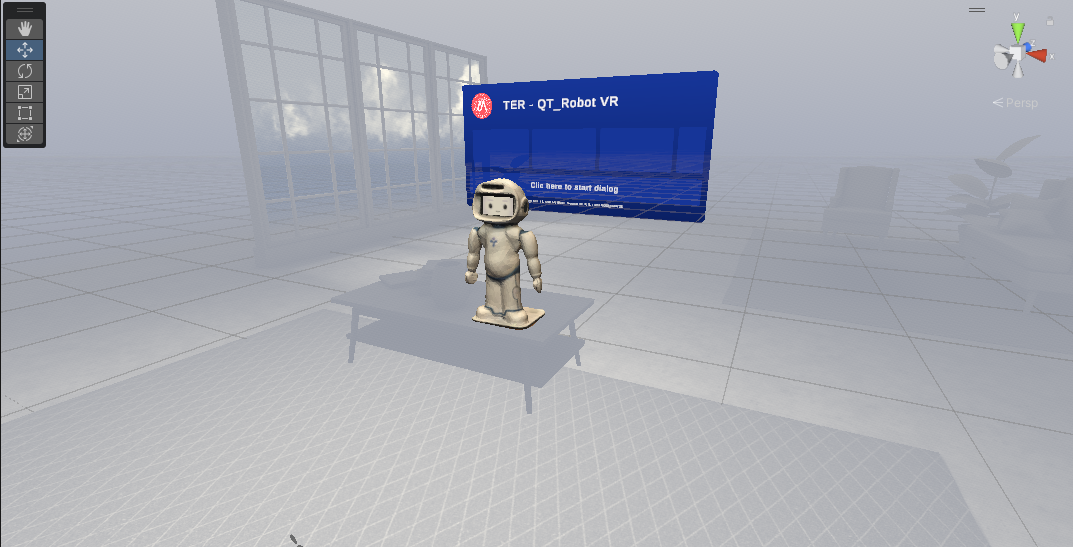
\includegraphics[height=7cm]{Figures/Scene_3D.png}
\caption{Screenshot of the final scene}
\end{figure}

\subsubsection{Dialogue}
The integration of Meta's API also enabled us to record a response from the user. Indeed, before we came up with the idea of the Wizard of Oz experience, it was based on a simple dialogue between the robot and the user. We chose to detect the user's voice in order to retrieve the text and pass it to ChatGPT using the OpenAI API to retrieve a response to give to the user. After a few tests, we noticed that users' feelings depended very much on the answer given by ChatGPT, which would have biased the results of the experiment. \\
\\
To ensure a match between the robot and VR experience, we pre-recorded the QT Robot's answers and played them back in the Unity scene. When the experimenter plays a question, the recording corresponding to the question is played.\\

\begin{figure}[!h]
\centering
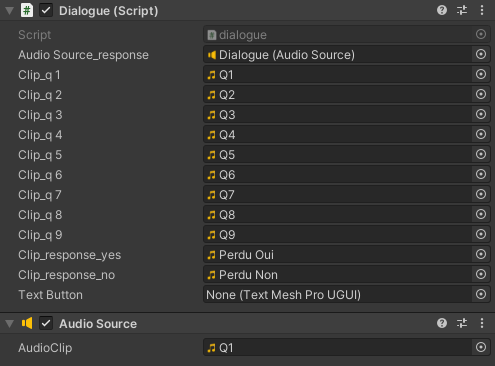
\includegraphics[height=7cm]{Figures/UnityDialogue.png}
\caption{Visualizing attributes on Unity}
\end{figure}

\begin{figure}[!h]
\centering
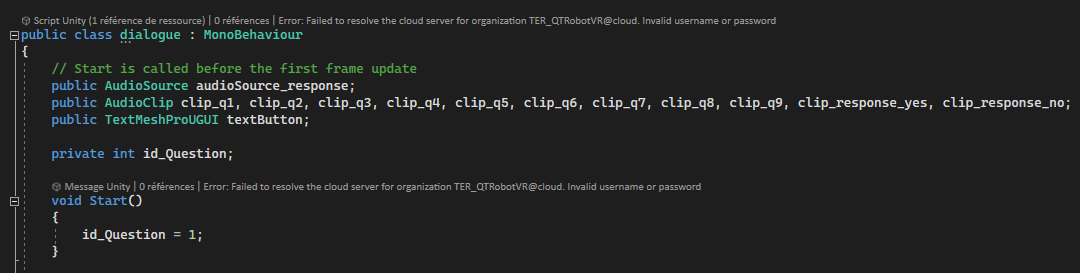
\includegraphics[height=3.5cm]{Figures/VSDialogue.png}
\caption{Declaring attributes in the script}
\end{figure}

\newpage
Here's how the experience is managed on the Unity side, with the example of launching responses. In figure 3.14, variables of type "AudioClip" have been declared and can be assigned in the Unity editor, as they are declared as "public". The rest of the script takes care of launching the desired audio file in the source audio, which is set to be played on the VR headset using the OVR Manager.
\chapter{Limitations and constraints}
In the course of our project, we were faced with several limitations and constraints that influenced our progress and our ability to achieve our objectives. These challenges added further complexity to our work and required proactive management to overcome them.\\

\subsection{The robot}
First of all, the lack of resources available online to solve the specific problems we encountered with the QTrobot was a big obstacle. Indeed, there is very little help or documentation available to guide us. This meant that our learning curve was slowed down enormously, as we had to spend a lot of time searching for relevant information and solving problems by trial and error.\\
\\
\\
\begin{minipage}{.65\textwidth}%
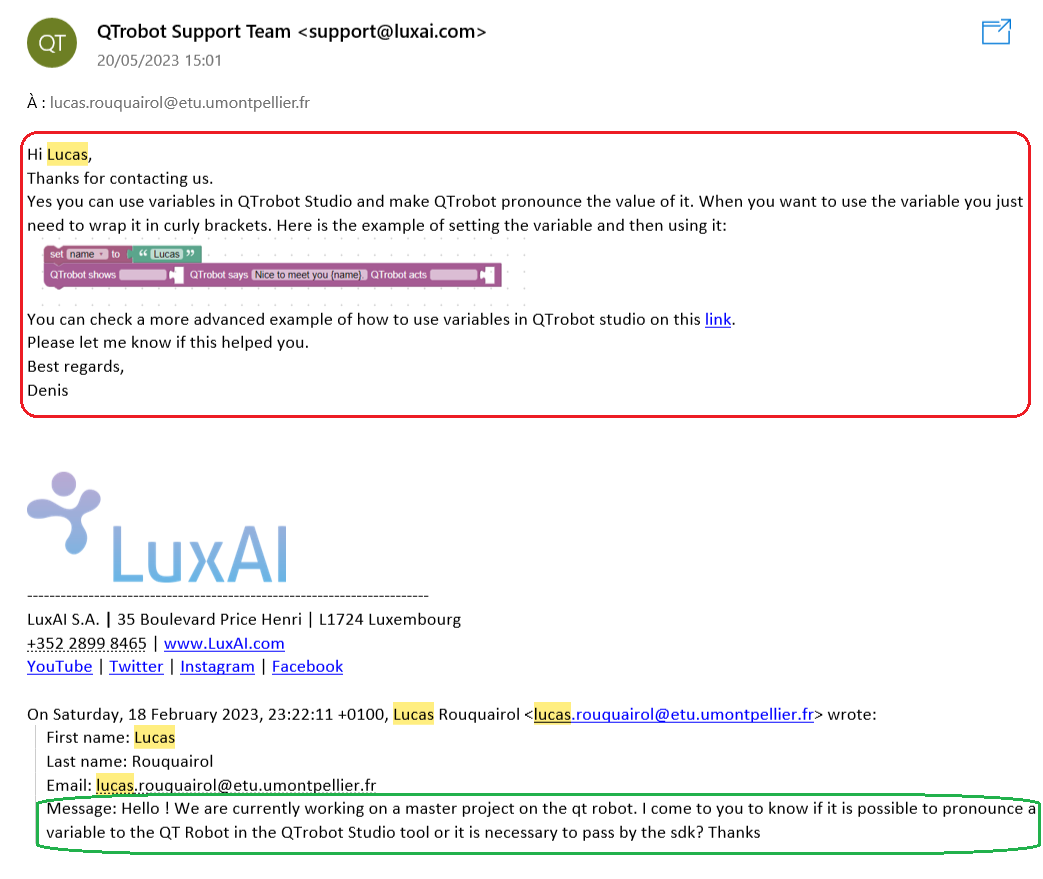
\includegraphics[width=\textwidth]{Figures/qtsupportemail.png}
\captionof{figure}{Exchange with support}
\end{minipage}%
\hfill
\begin{minipage}{.33\textwidth}%
When we encountered more complex problems, we had to call on technical support via e-mail. Unfortunately, support response times were sometimes slow, resulting in further delays in resolving our problems. We had to manage our impatience while continuing to work autonomously wherever possible.\\
\end{minipage}%
\newpage
In addition, limited access to the robot was a major obstacle. The robot was stored in the secretariat of Building 16, which meant that it could only be accessed during the secretariat's opening hours, i.e. only on weekdays and before 5pm. What's more, as other teams also had to use it, we had to plan our usage time carefully. These constraints led to delays in our development schedule and limited our scope for experimentation. We had to organize ourselves efficiently to optimize every moment of access to the robot.\\
\\
\subsection{The time}
The partial availability of our team was a constant challenge. Indeed, due to various constraints, not all team members were available simultaneously. This complicated coordination and collaboration within the group, sometimes resulting in additional delays and uneven distribution of tasks.\\
\\
What's more, we were under considerable time pressure. We had to finalize the project quickly in order to present it to the participants. This put additional pressure on the team, limiting our ability to make in-depth improvements or explore advanced QTrobot functionalities. We had to focus on the essentials to meet the deadline.\\
\\
\subsection{The experience}
Finally, the difficulty of bringing together all the participants in the experiment on the same day was a major challenge to ensuring effective communication and collaboration. Constraints related to individual availability led to delays and absences of some participants, which had a direct impact on the overall progress of the project. To overcome this situation, we had to maintain constant coordination and make frequent adjustments to the schedule. We had to be flexible and responsive in order to find time slots that suited all participants, and this required careful management of everyone's schedules. Despite these logistical challenges, we maintained an open and regular dialogue with all participants, ensuring that everyone was informed of developments and could actively contribute to the experience.\\
\\

\chapter{Experience}
\section{Wizard of Oz background}
\subsection{Definition and relevance}
The experiment is based on the "Wizard of Oz" concept of human-robot interaction. In reality, the QT-robot is not able to hear the participants or make autonomous decisions in the "Neither Yes nor No" game. Instead, we, as operators, manually controlled the course of the game and the robot's responses.

As participants interacted with the robot, we stood behind the scenes and pressed buttons to move the robot on to the next question. In addition, we also determined whether the participant's answer was "yes" or "no" by pressing separate buttons for each response. This enabled us to provide an appropriate response from the robot, saying "yes" or "no" to indicate whether the participant had lost or not.

The aim of this approach was to simulate a realistic interaction between the participants and the robot, making them believe that the robot was actually capable of understanding their responses and making decisions accordingly. Using the concept of the "Wizard of Oz", we were able to observe participants' reactions and behaviors in the face of this apparently autonomous interaction with the robot.\\
\subsection{Implementation in the VR experience}
It was easier to guarantee the context of the Wizard of Oz in VR, as the subject is fully immersed in the virtual scene. The Oculus headset works with two joysticks (one for each hand), both of which have buttons for interacting with the scene. The right joystick, held by the subject, allows him or her to launch the dialog when ready, while the left joystick allows the experimenter to skip answers or launch the end dialog if the subject has said "yes" or "no". This stratagem allows the subject to be immersed in the experiment without being aware of the "Wizard of Oz" context.
\\
\begin{figure}[!h]
\centering
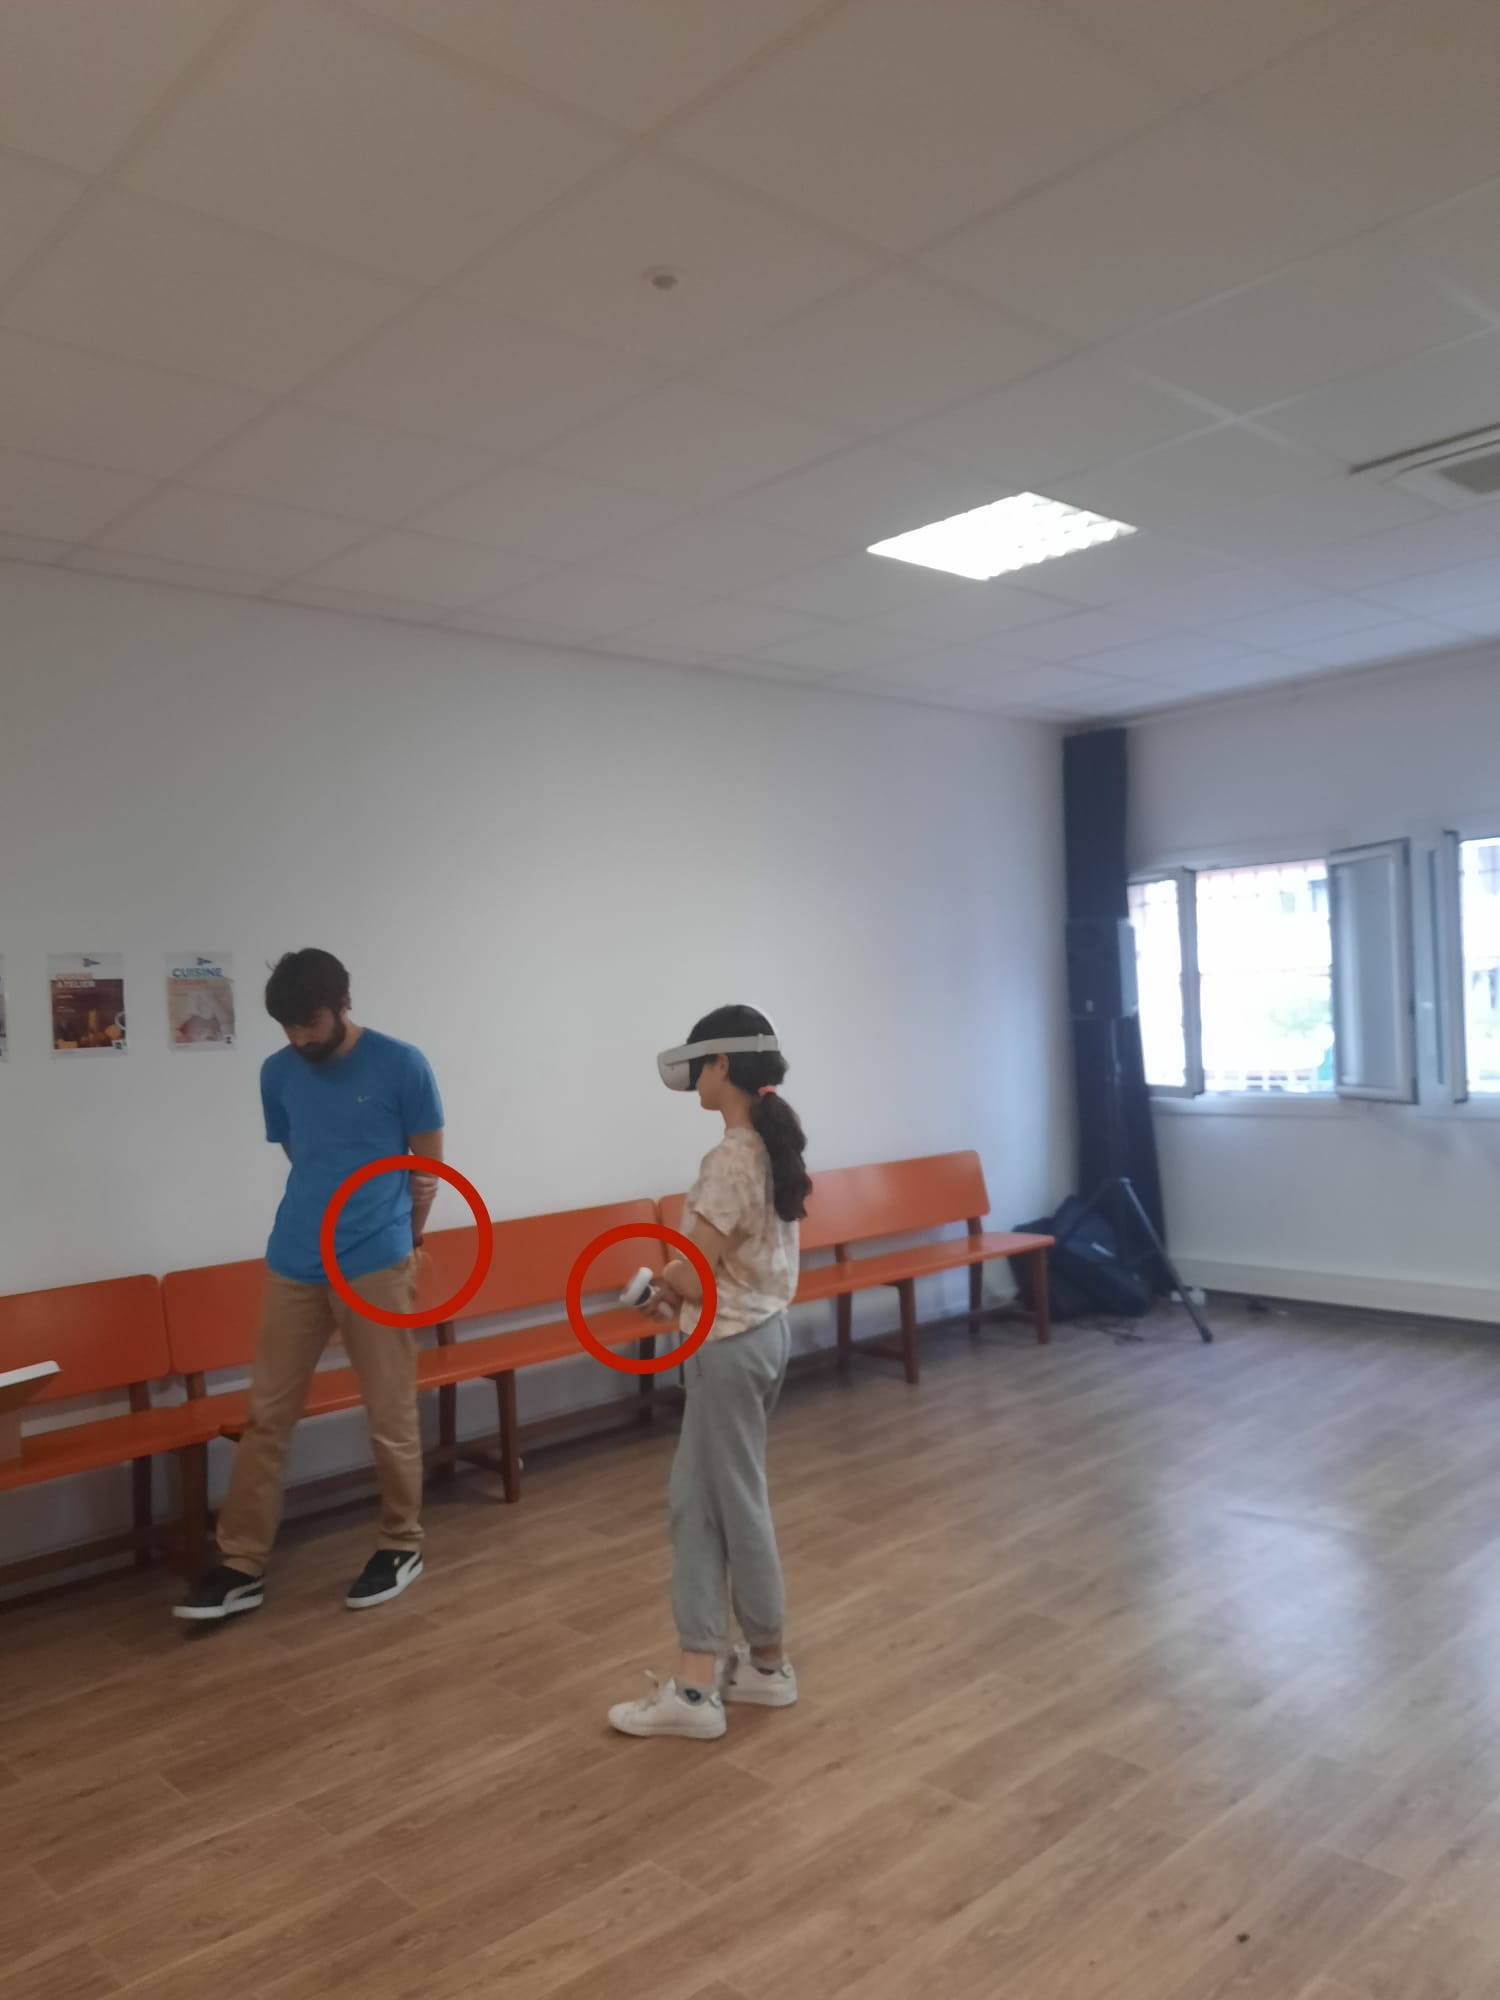
\includegraphics[height=7cm]{Figures/Oz_VR.jpeg}
\caption{Control distribution system in VR}
\end{figure}\\

\subsection{Integration with robot physics experience}

To set up the "Wizard of Oz" context in the physics experiment, it was necessary to use trickery so that the participants didn't realize that the experimenter was playing the questions. Indeed, it was necessary to use a keyboard to launch the dialogue, switch from one question to another, and trigger a specific message when one of the participants used the words "yes" or "no". To divert the participants' attention and prevent them from realizing that everything was being done manually by the person to their right, the robot was positioned opposite the keyboard and the screen displaying the robot's script.

In addition, the window displaying the script was reduced to its minimum size on the screen, ensuring that subjects did not notice it. This configuration helps create the illusion of autonomous interaction between participants and the robot, reinforcing immersion in the experience.
\begin{figure}[!h]
\centering
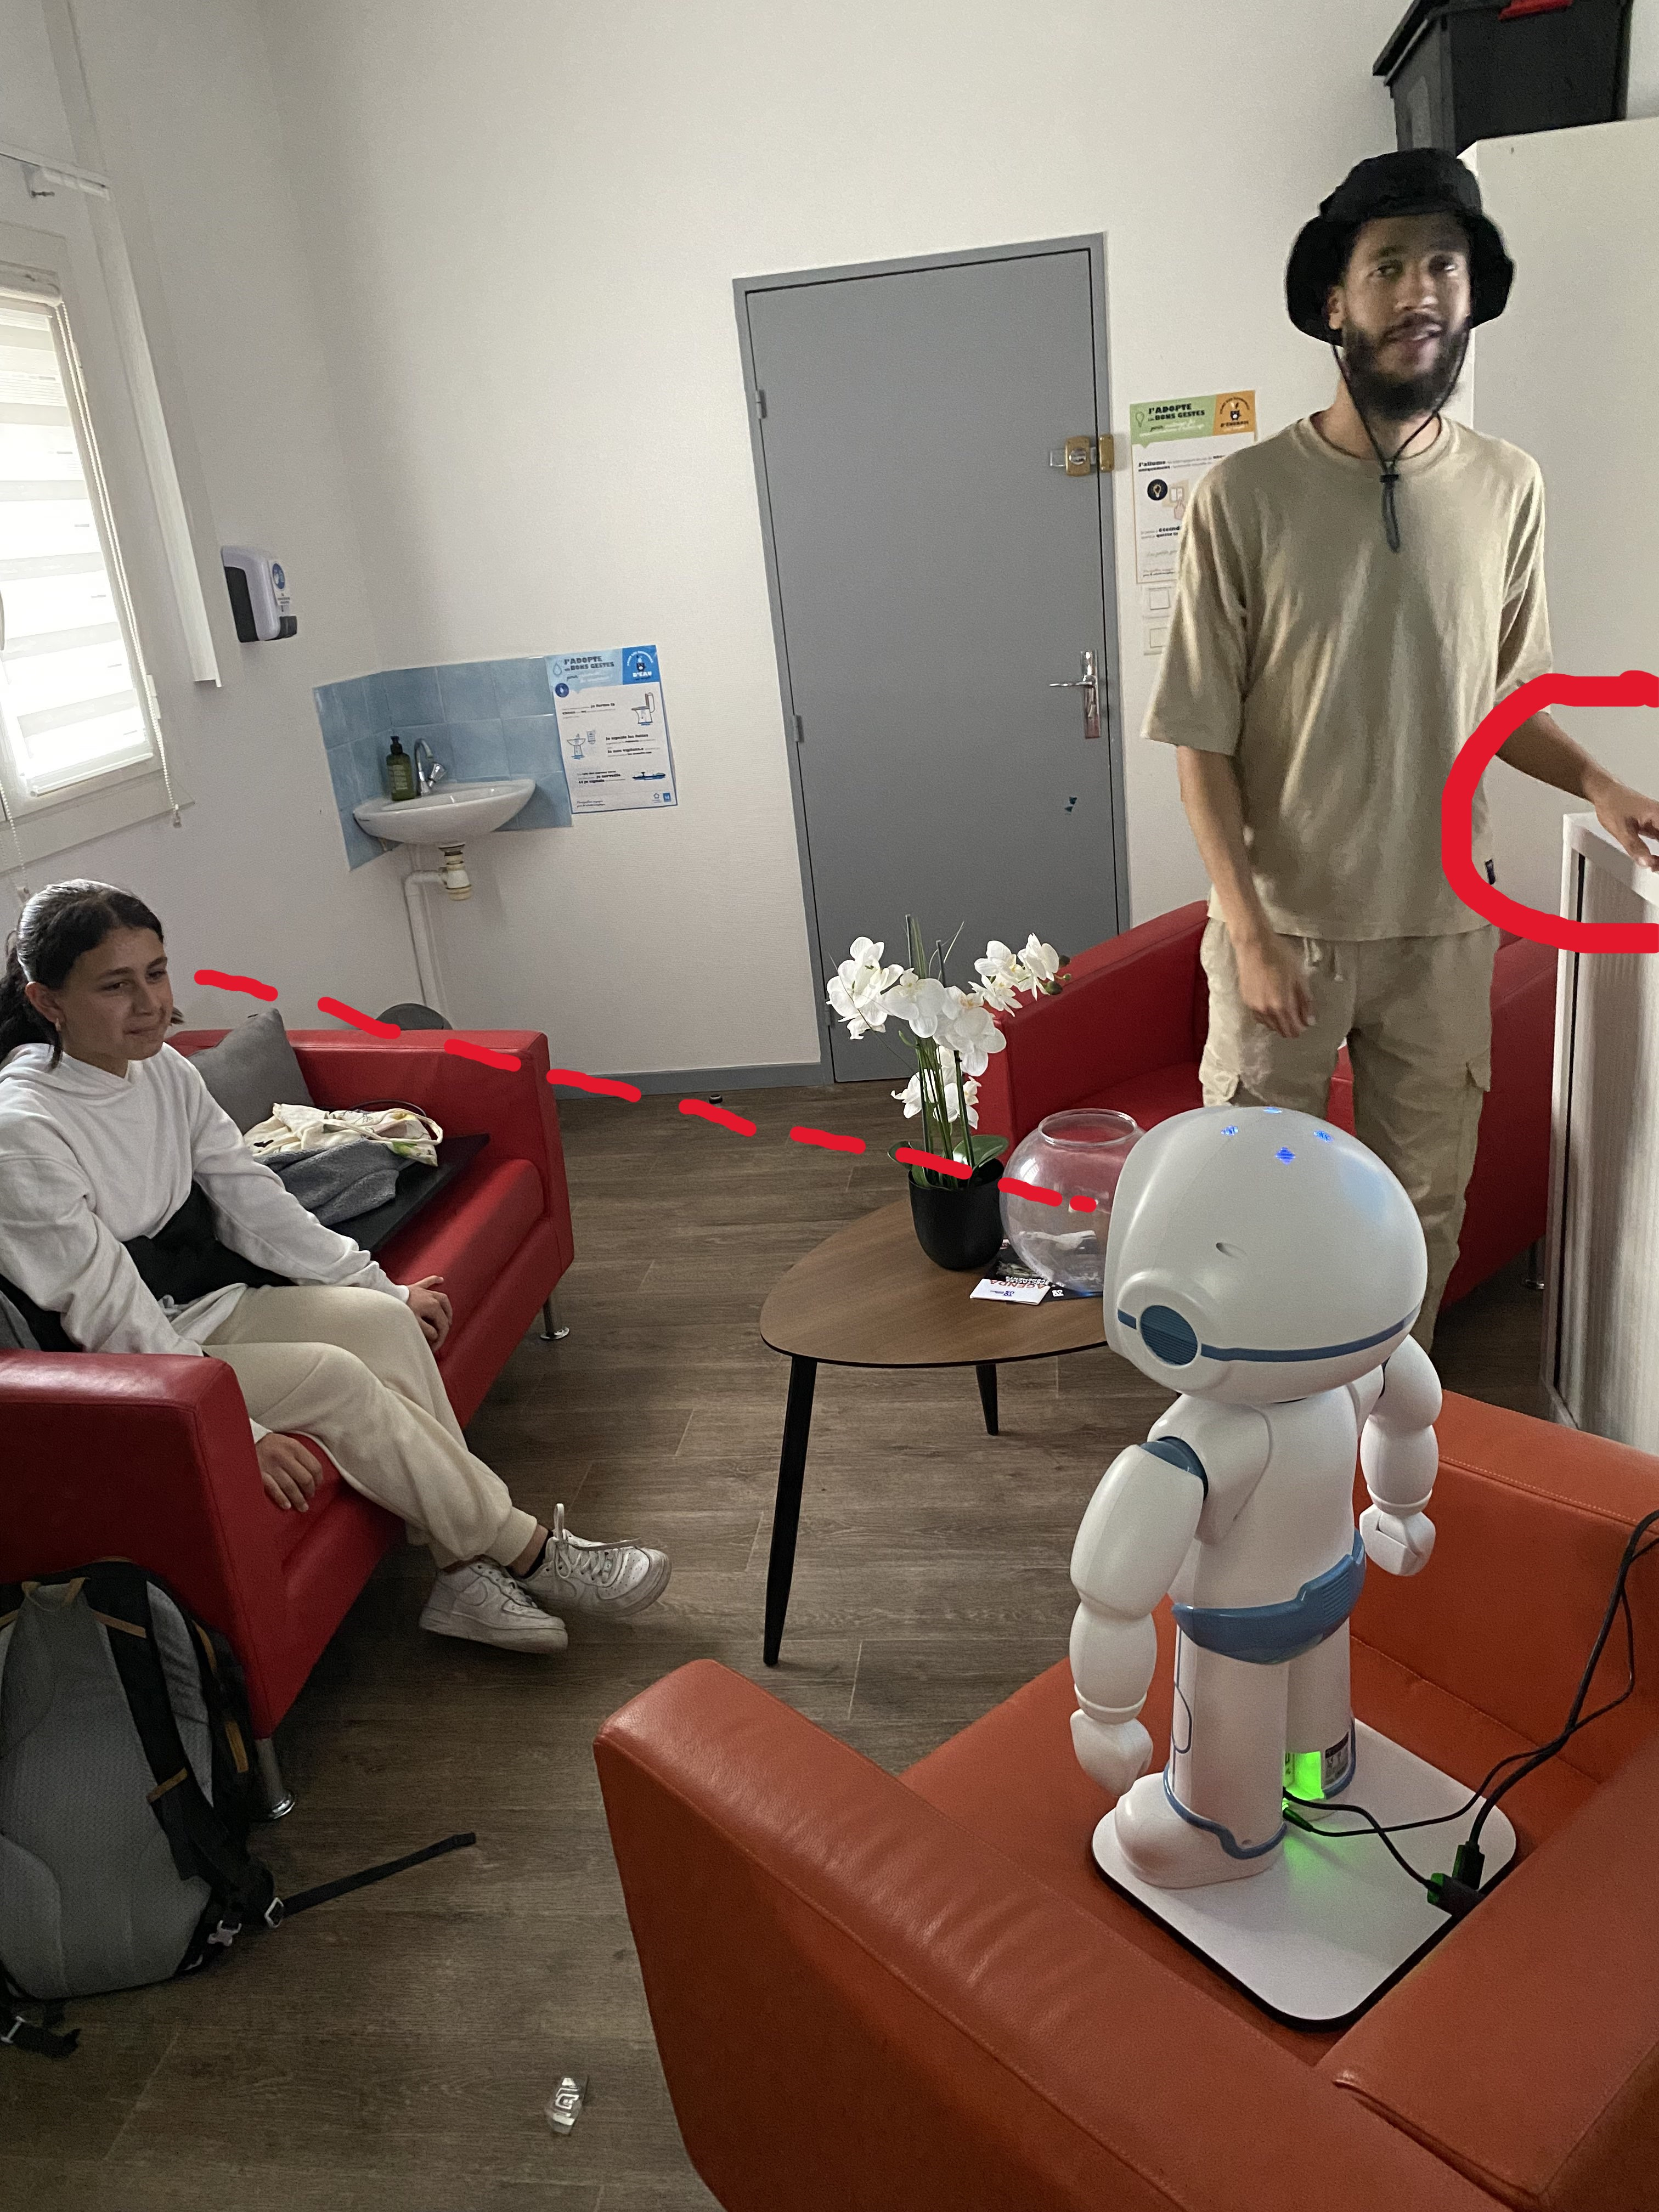
\includegraphics[height=7cm]{Figures/magicien3.jpg}
\caption{Robot control system}
\end{figure}\\

\section{The process}
\hspace{\parindent} In order to provide the best possible answer to the question raised by the subject, we carried out an experiment to study human-robot interaction using the QT-robot in a game of "Neither yes nor no". The main aim of the experiment was to assess the impact of the robot's embodiment on interaction and engagement.\\
\\
We organized the experiment in two distinct stages. The first stage was conducted with students from our faculty, while the second stage took place in a home for all, in collaboration with a tutoring association for children from a background where most of them had never experienced virtual reality (VR) or even had the opportunity to see a robot like QT-robot. The subjects were divided into two groups, one for the robot experience and the other for the VR experience.\\
\\
After accepting the conditions of the experiment and processing the results, the first group of participants were invited to interact with the QT-robot in a game of "Neither Yes nor No". The aim was for participants to hold a conversation with the robot without uttering the words "yes" or "no". The robot was programmed to ask a series of questions and engage the participants in discussion, encouraging them to answer without using the forbidden words. If a participant managed to keep the conversation going without saying "yes" or "no" for a predetermined length of time, he or she was deemed the winner. Winners received rewards in the form of a sweet and a cake, while losers went home empty-handed.\\
\\
The second group was invited to reproduce the same "Neither Yes nor No" game, but this time using virtual reality (VR). Participants wore a VR headset that enabled them to view and interact with the QT-robot virtually. In this way, we were able to observe the differences in feel and engagement between physical interaction with the robot and virtual interaction with its VR representation.
\\
At the end of each experiment, participants were invited to complete a questionnaire specially designed for this study. They could access it by scanning the QR code provided using their phone for adults, and by filling in the paper questionnaire for children. The purpose of the questionnaire was to gather their impressions and feelings about their experience with the robot or the VR representation. The questions on the questionnaire were adapted for children to ensure that they were easy to understand.\\
\\
\begin{figure}[!h]
\centering
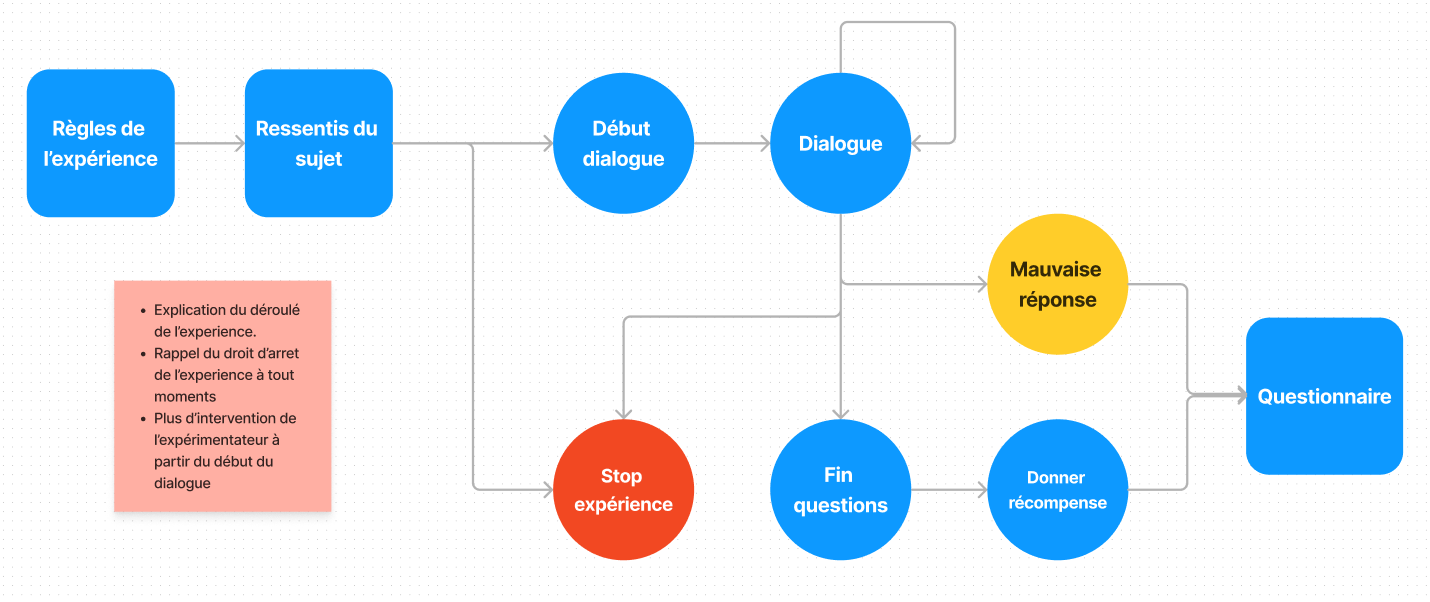
\includegraphics[width=2\textwidth, height=0.30\textheight,keepaspectratio]{Figures/Experience_Roadmap_Resize.png}
\caption{Experience roadmap}
\end{figure}
\\
Analysis of the responses obtained from the questionnaires will enable us to compare the differences in feeling between the two experiences, and to assess the impact of embodiment on human-robot interaction.\\

\section{The participants}

For the experiment, our professor gave us permission to promote it to the faculty students. During a project management course, we had the opportunity to invite them to participate at a later date. We also promoted the experiment on our university's Discord server. The experiment took place directly on the faculty campus. The participants were mainly students between the ages of 18 and 26, from a wide range of courses. Thanks to the Discord broadcast, we also attracted participation from students of other backgrounds and ages.\\
\\

\begin{figure}[htp]
    \centering
    \begin{minipage}[c]{0.5\textwidth}
        \centering
        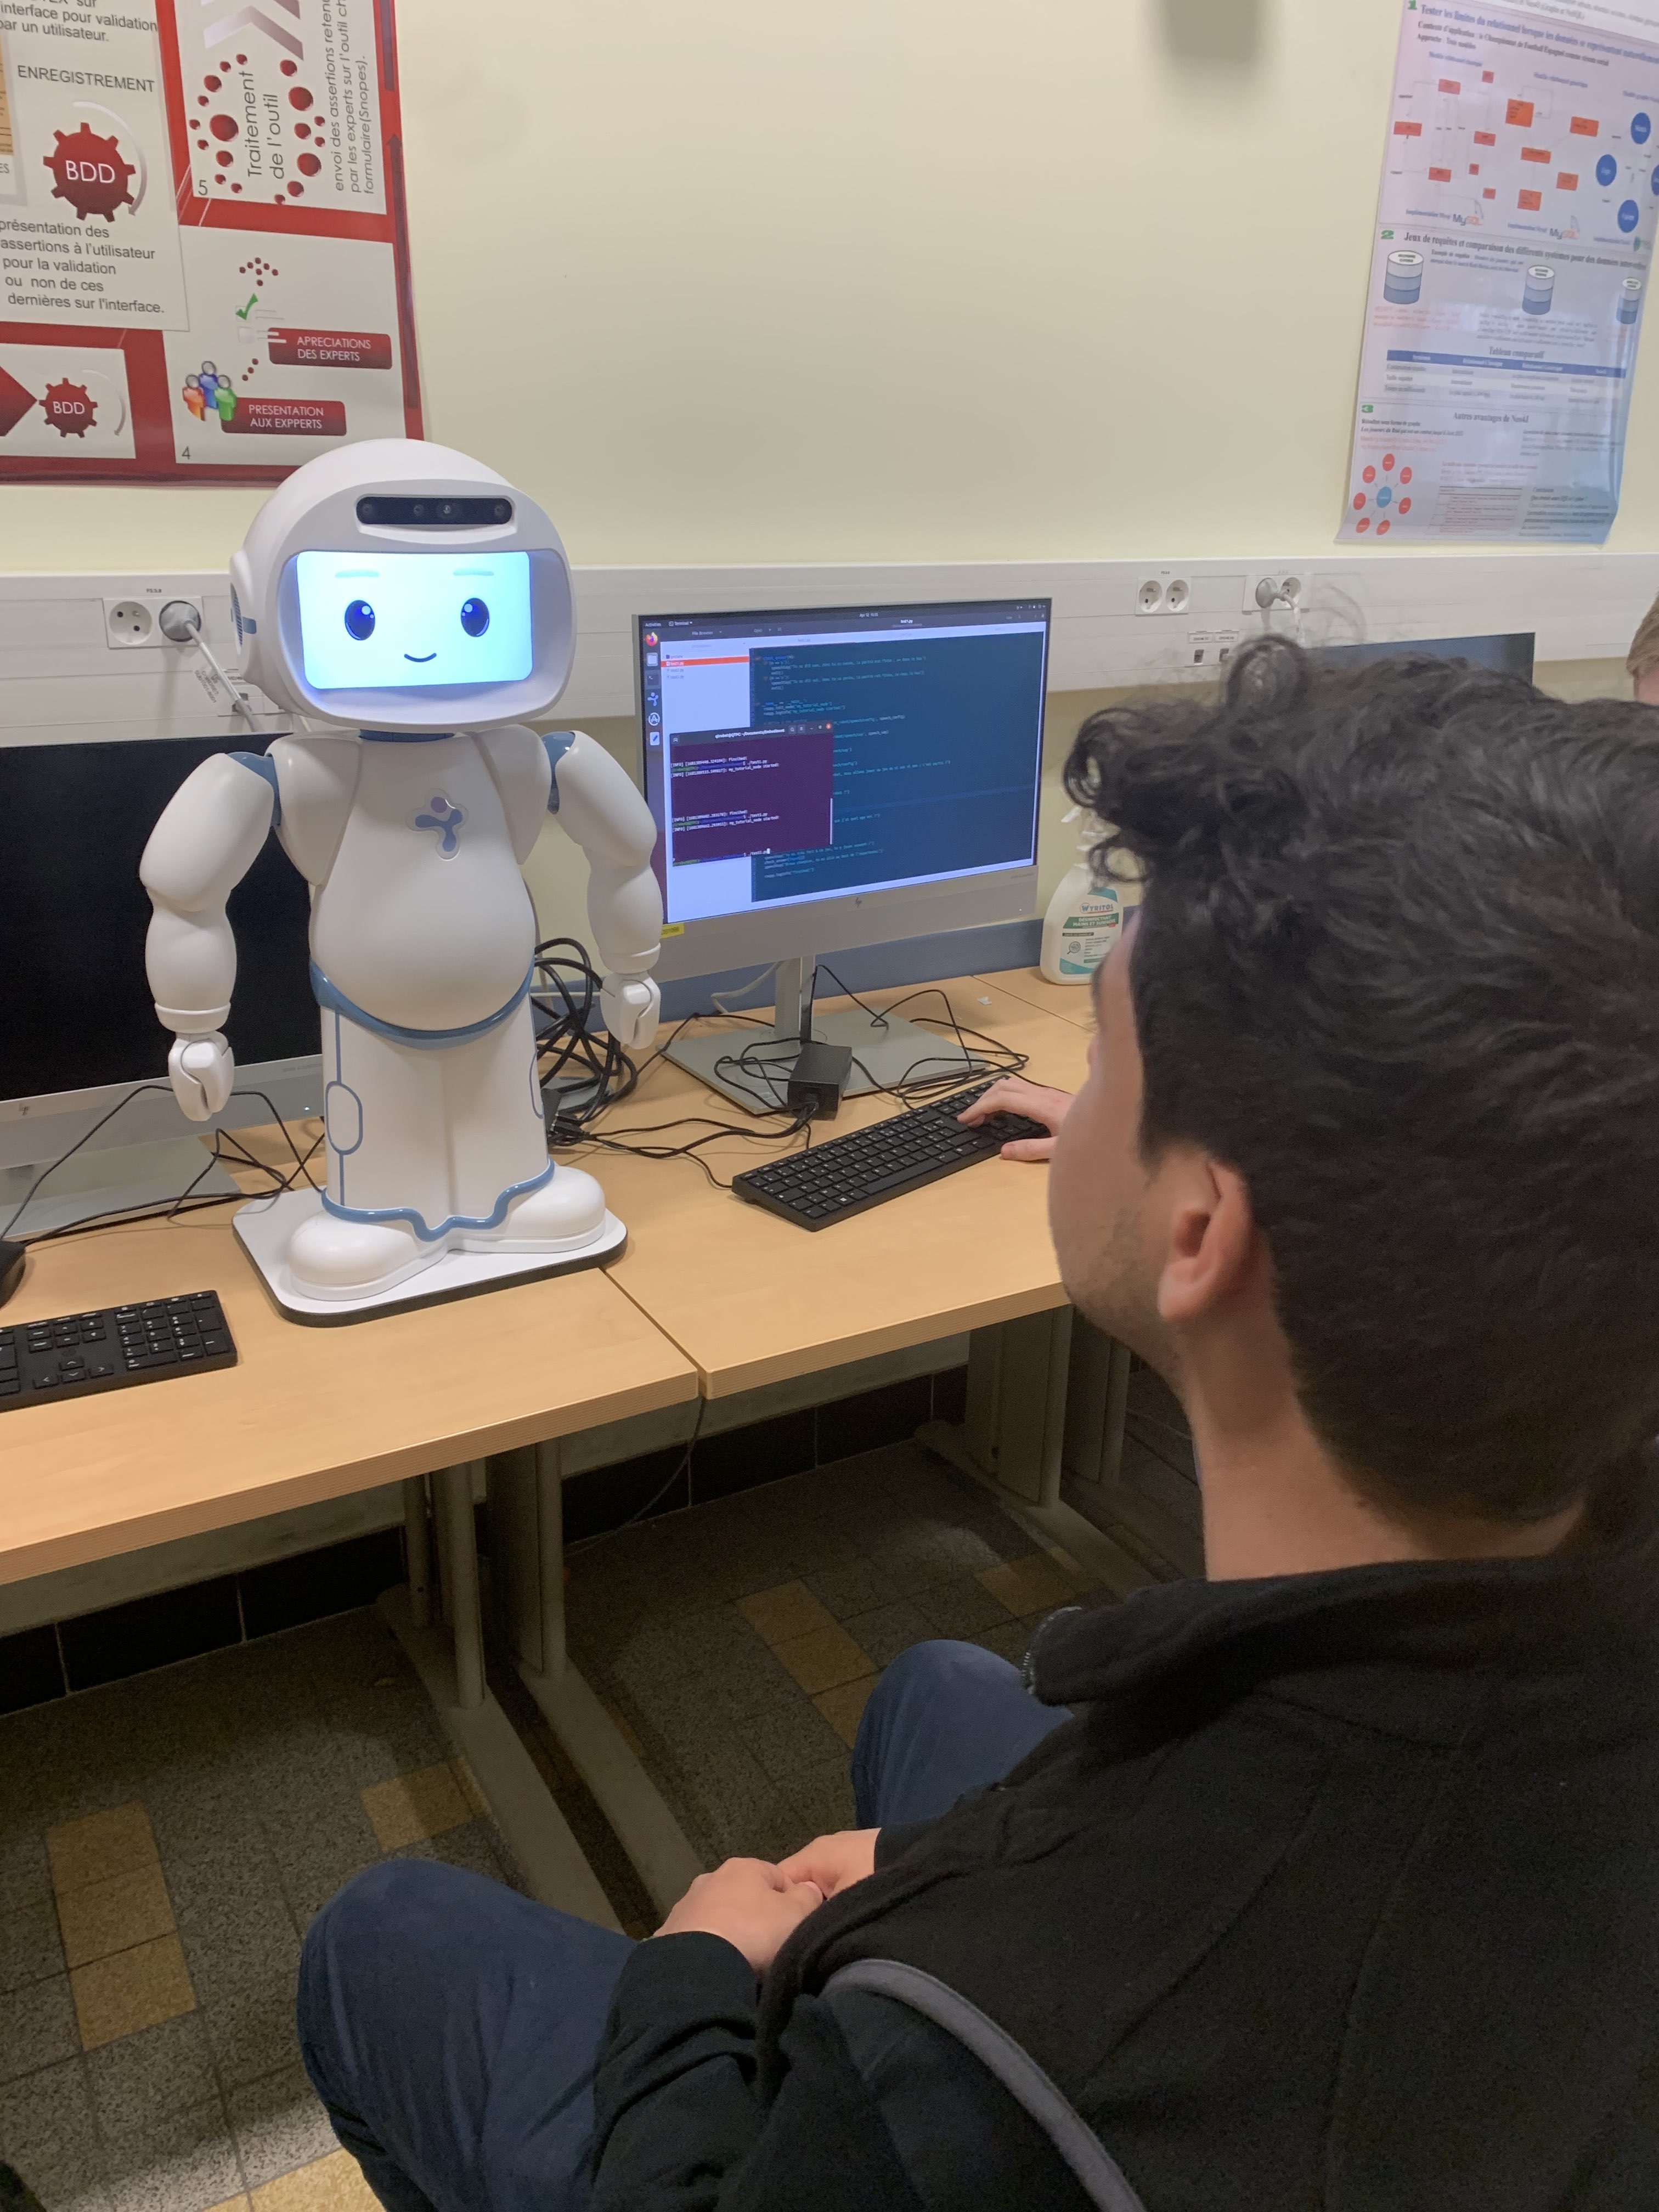
\includegraphics[width=1.0\textwidth, height=0.3\textheight,keepaspectratio]{Figures/ryan.jpg}
        \caption{Physical adult experience}
    \end{minipage}%
    \begin{minipage}[c]{0.5\textwidth}
        \centering
        \includegraphics[width=1.0\textwidth, height=0.3\textheight,keepaspectratio]{Figures/Adulte_VR.jpg}
        \caption{Adult VR Experience}
    \end{minipage}
\end{figure}
\newpage
For the experiment with the children, knowing that one of the people in our group is a member of a children's tutoring association, we obtained permission from her tutor to carry out and present the experiment to the children of this association. We took the QT-robot, VR headset and candy to the children's home. There, we were able to connect the QT-robot to a screen and launch the "Neither Yes nor No" game. The children taking part in the experiment were aged between 9 and 15, and generally had no experience of robots or virtual reality. As the children didn't have telephones, we prepared printed questionnaire sheets on which they answered the questions.\\
\begin{figure}[htp]
    \centering
    \begin{minipage}[c]{0.5\textwidth}
        \centering
        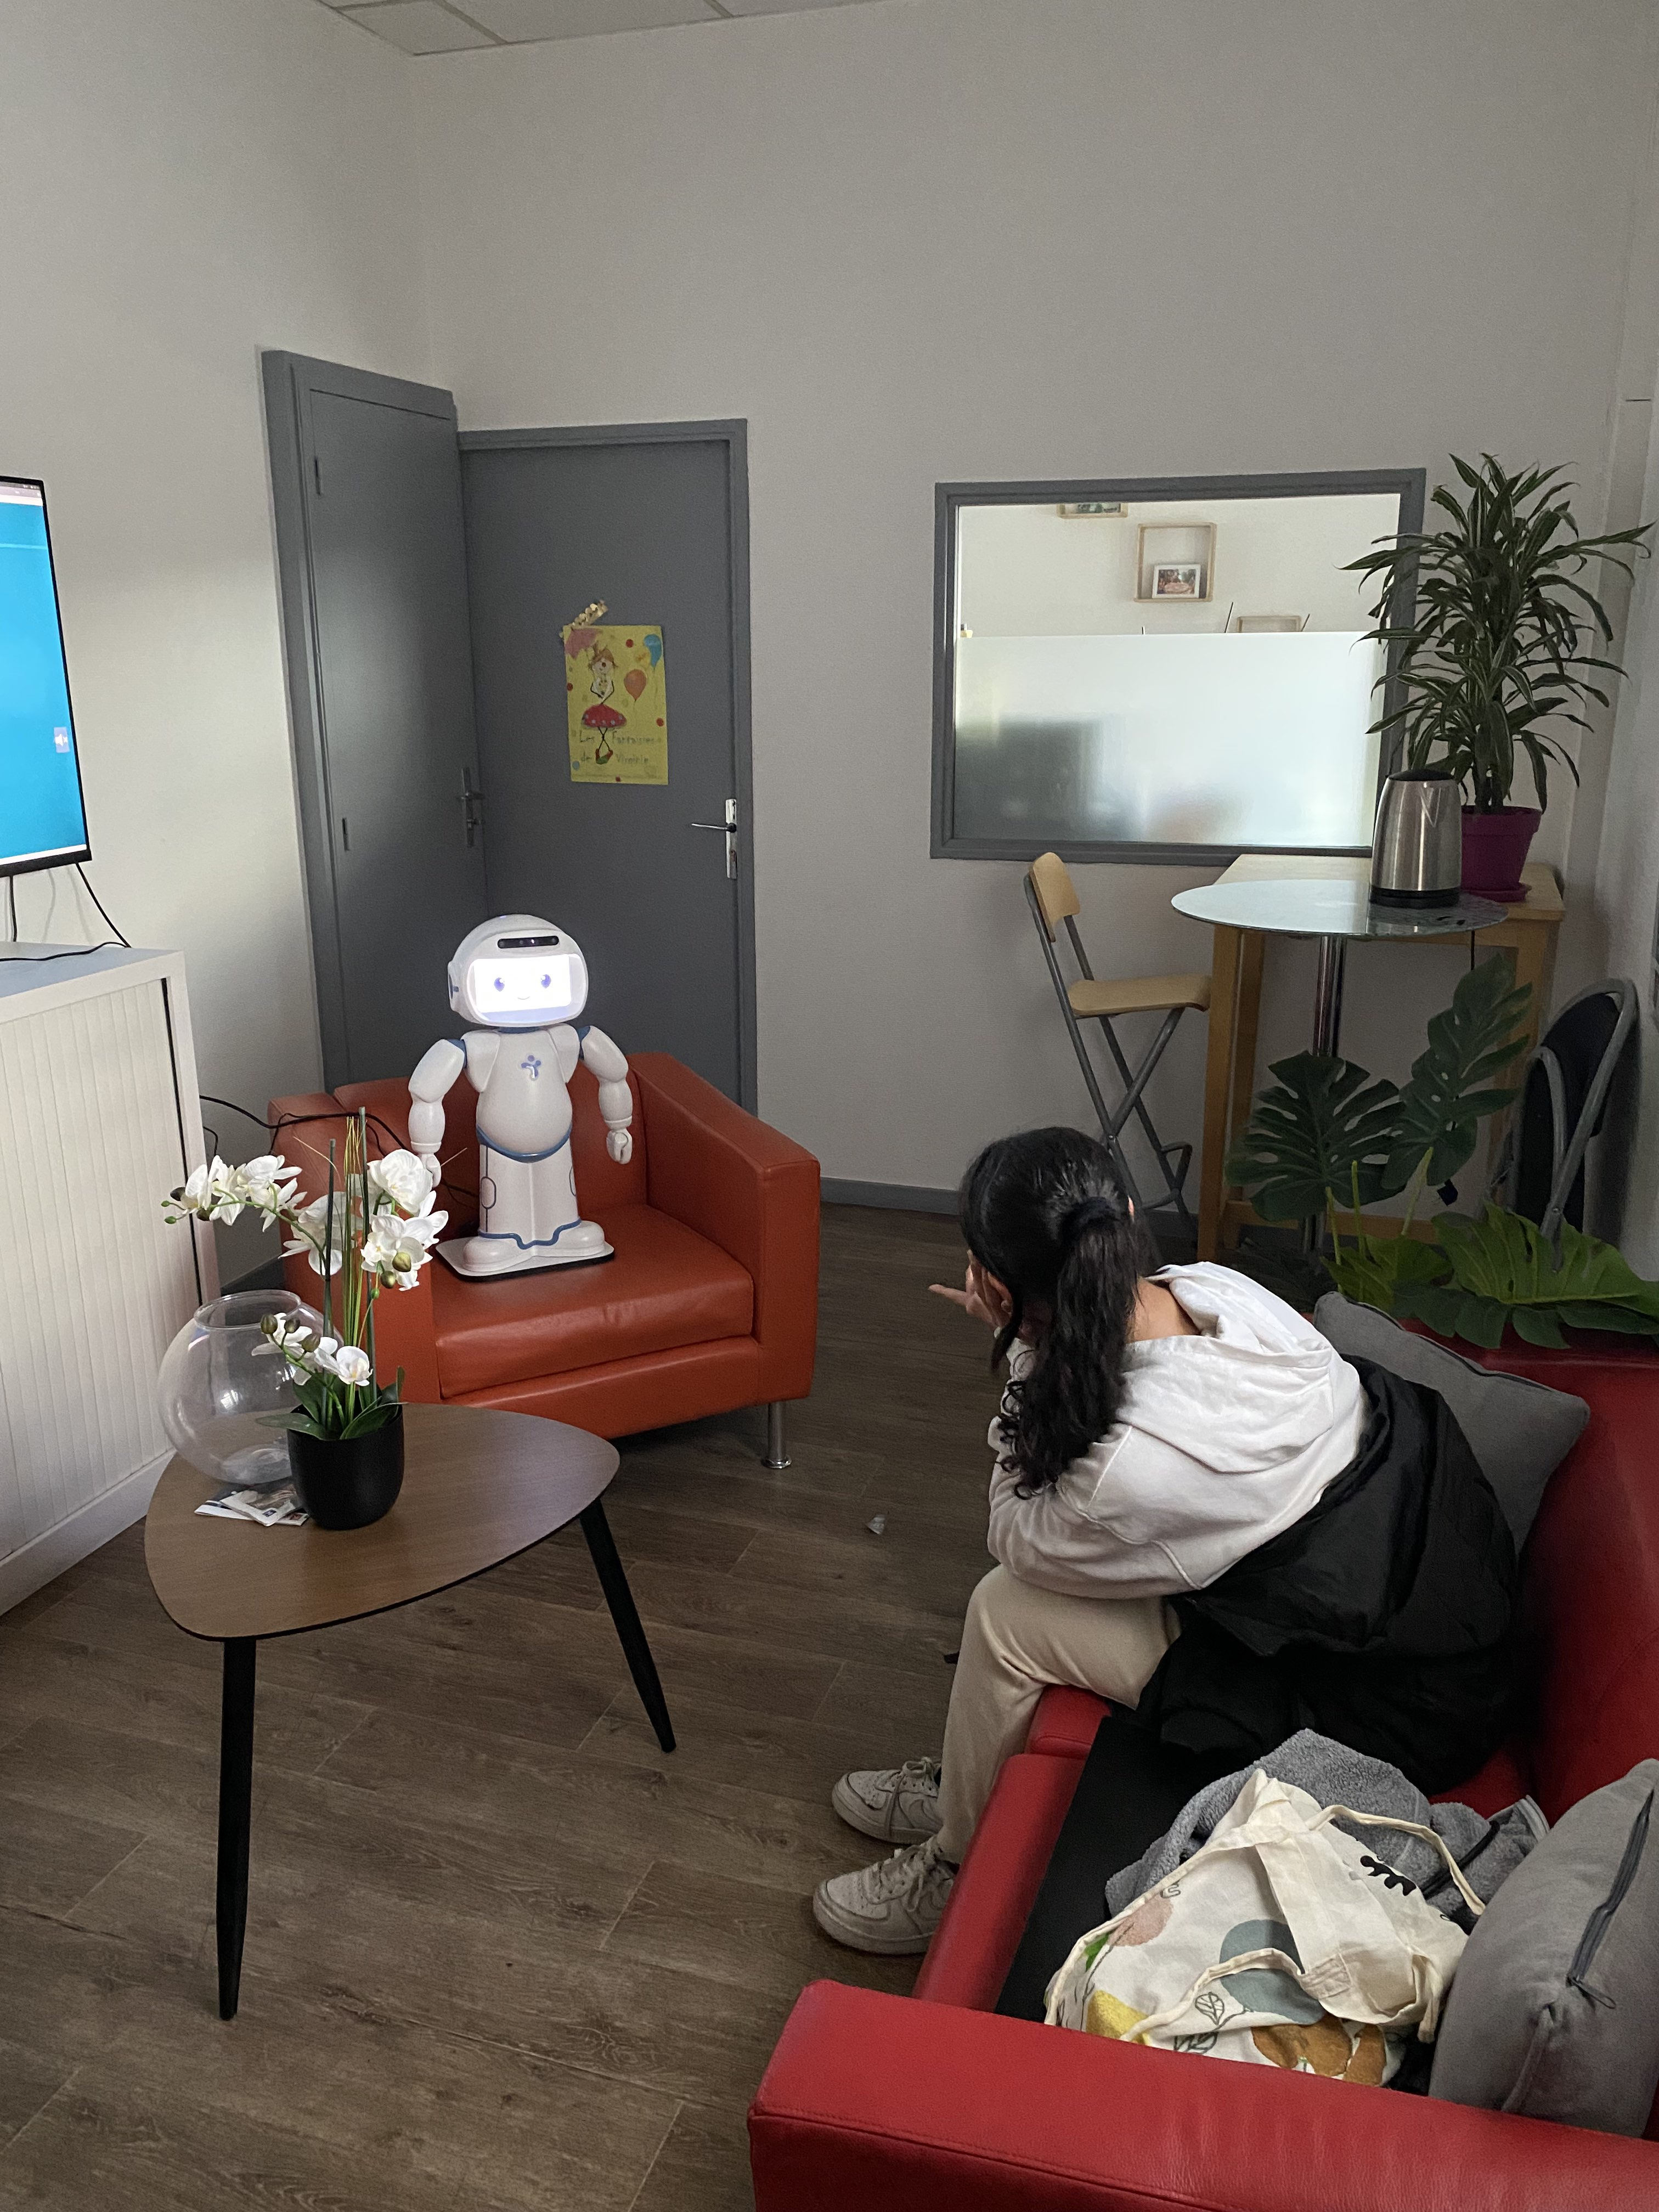
\includegraphics[width=1.0\textwidth, height=0.3\textheight,keepaspectratio]
        {Figures/ryma.jpg}
        \caption{Physical child experience}
    \end{minipage}%
    \begin{minipage}[c]{0.5\textwidth}
        \centering
        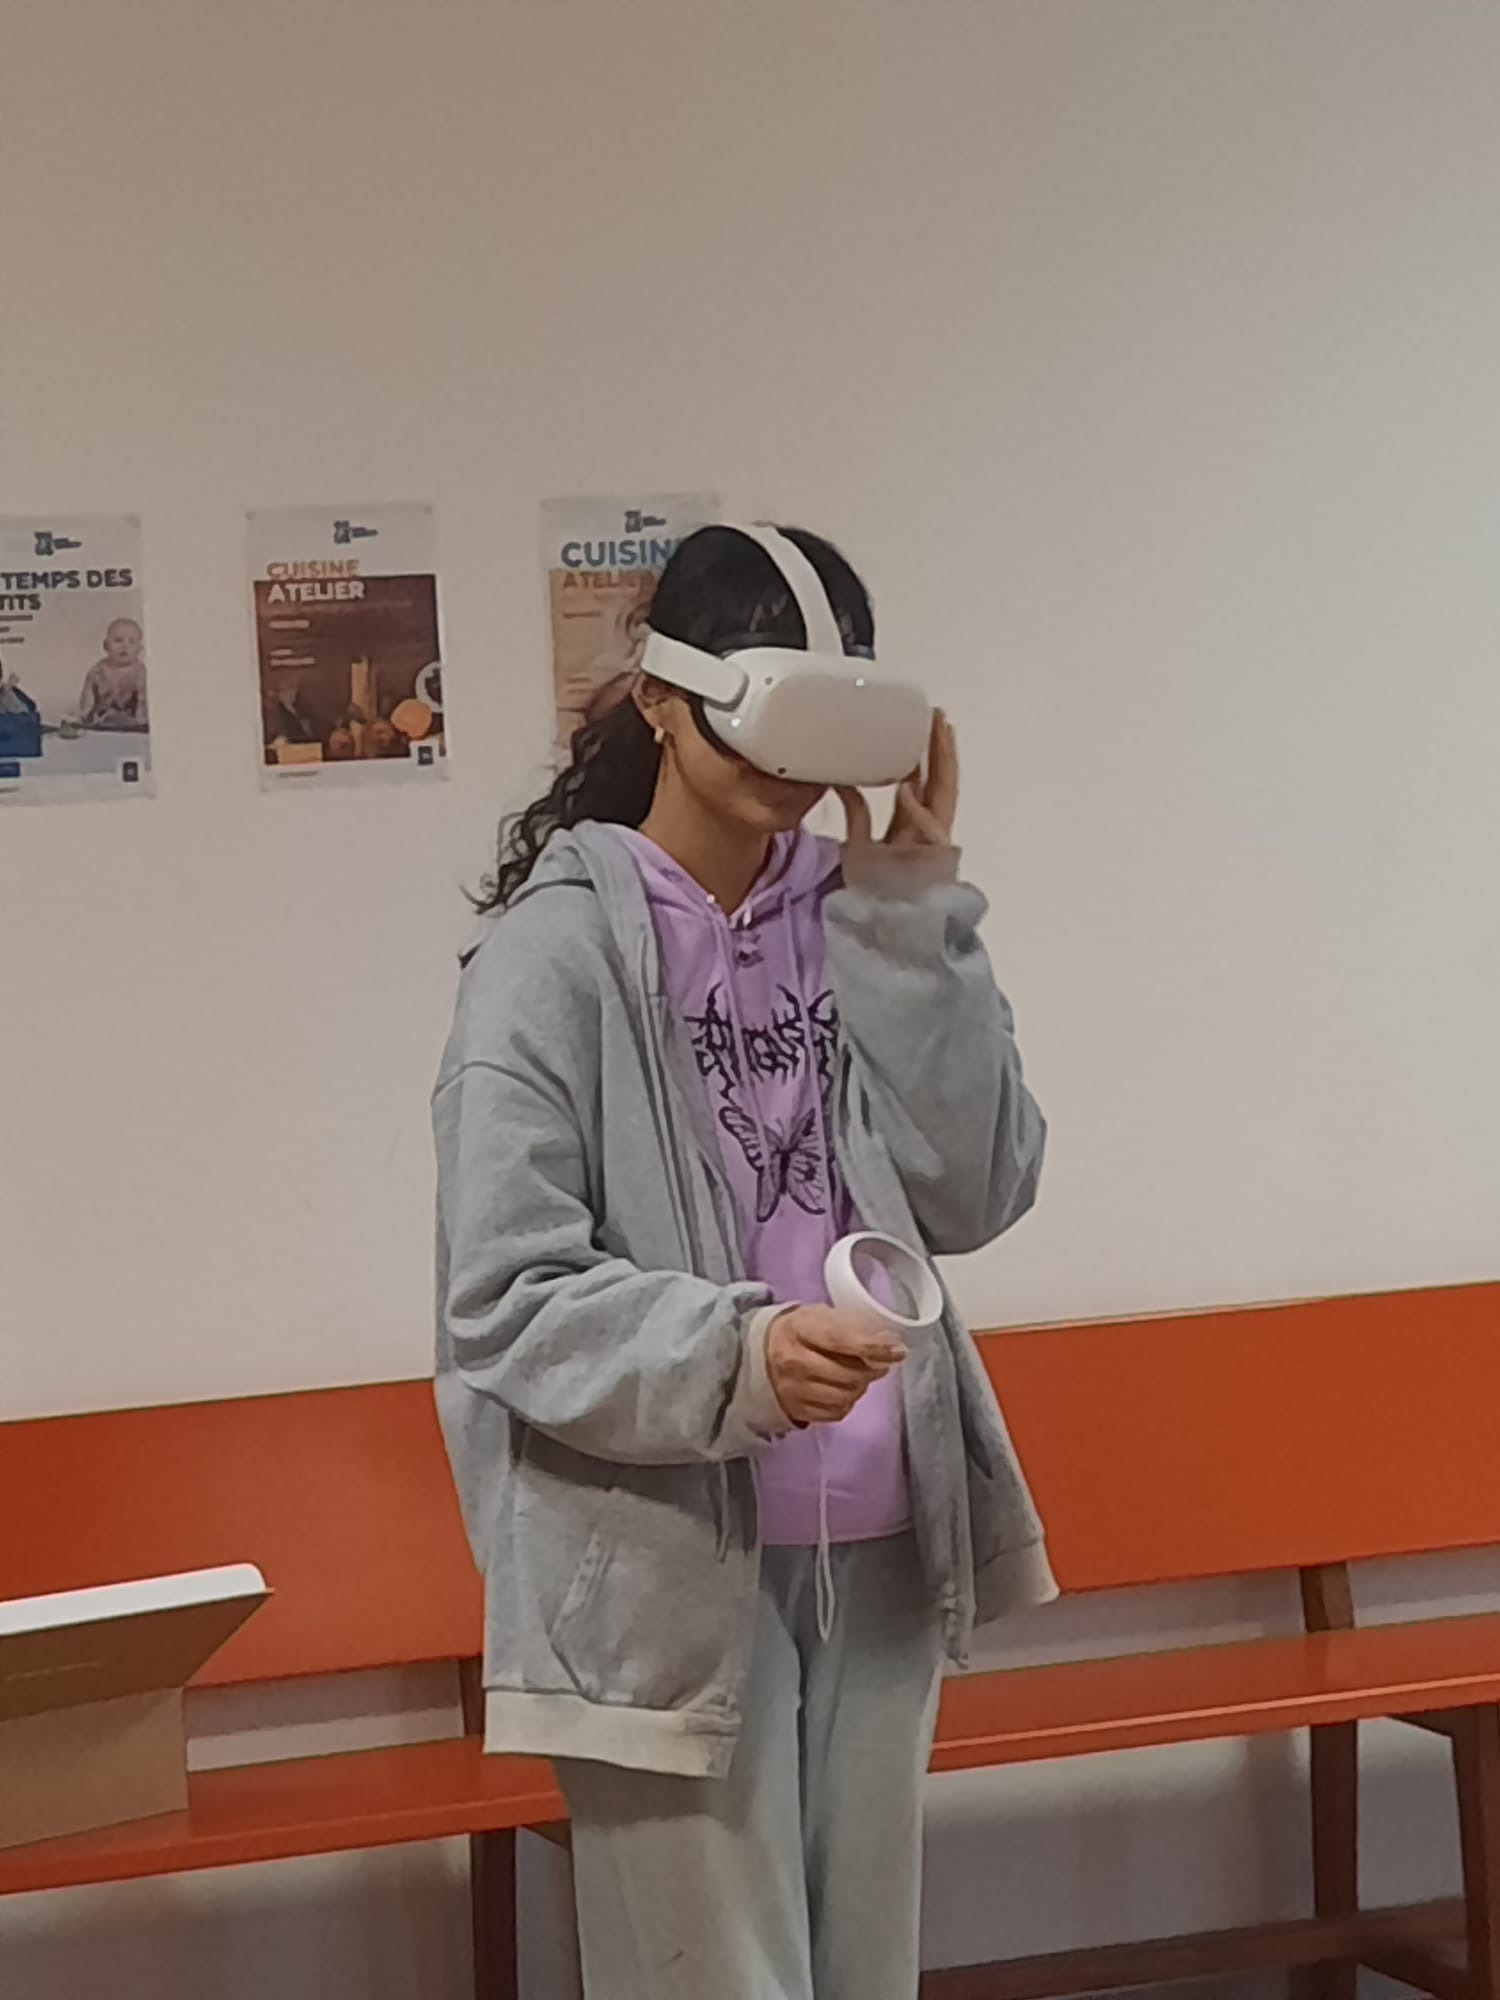
\includegraphics[width=4\textwidth, height=0.3\textheight,keepaspectratio]{Figures/yasmina.jpg}
        \caption{Children's VR experience}
    \end{minipage}
\end{figure}
\\


\chapter{Data analysis}

We were privileged to have the active participation of 20 adults and 9 children in our experiment. We will present the data in two formats: percentages for "yes"/"no" responses, and averages for responses out of five. The same questions are asked of subjects who have undergone the virtual reality experience as well as those who have physically interacted with the robot.\\
\subsection{Adults}

    \subsubsection{Did you feel empathy for the robot?}
    \begin{minipage}{.5\textwidth}%
    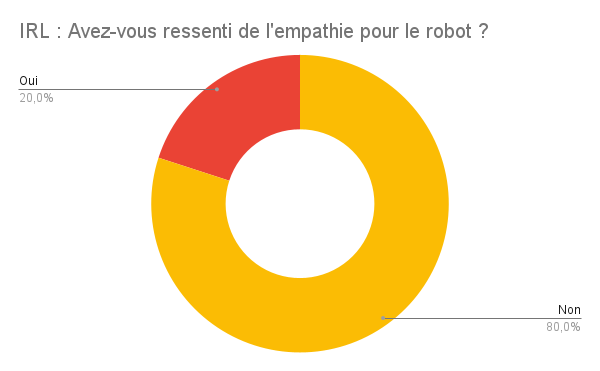
\includegraphics[width=\textwidth]{Datas/IRL _ Avez-vous ressenti de l'empathie pour le robot _.png}
    \captionof{figure}{Physics}
    \end{minipage}%
    \begin{minipage}{.5\textwidth}%
    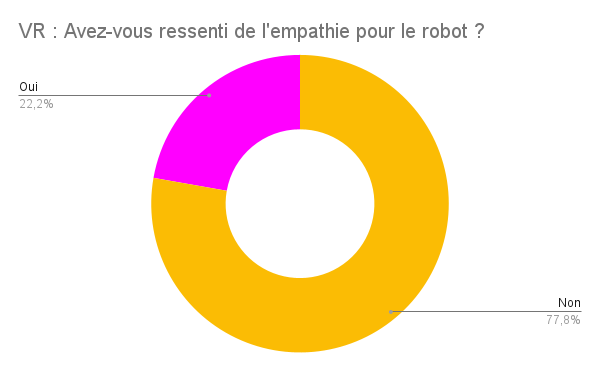
\includegraphics[width=\textwidth]{Datas/VR _ Avez-vous ressenti de l'empathie pour le robot _.png}
    \captionof{figure}{VR}
    \end{minipage}%
    \vspace*{0.5cm}
    
    \subsubsection{Did you get the impression that the robot had a distinct personality?}
    \begin{minipage}{.5\textwidth}%
    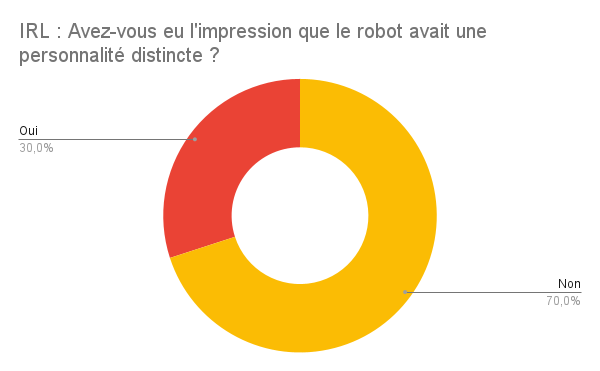
\includegraphics[width=\textwidth]{Datas/IRL_personnalite_distincte.png}
    \captionof{figure}{Physics}
    \end{minipage}%
    \begin{minipage}{.5\textwidth}%
    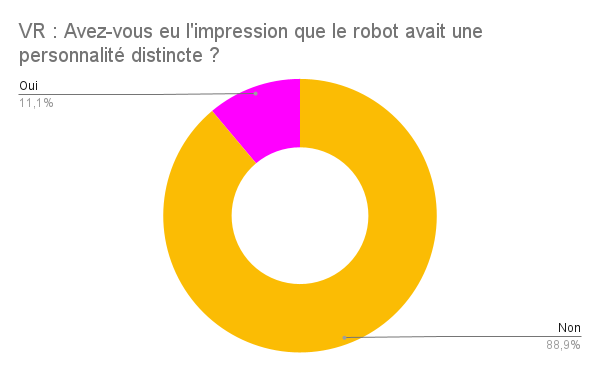
\includegraphics[width=\textwidth]{Datas/VR_personnalite_distincte.png}
    \captionof{figure}{VR}
    \end{minipage}%
    \vspace*{0.5cm}


    \subsubsection{Do you think the robot cheated during the game?}
    \begin{minipage}{.5\textwidth}%
    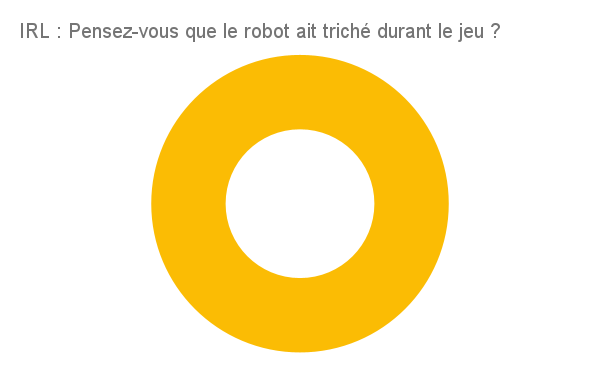
\includegraphics[width=\textwidth]{Datas/IRLtriche.png}
    \captionof{figure}{Physics}
    \end{minipage}%
    \begin{minipage}{.5\textwidth}%
    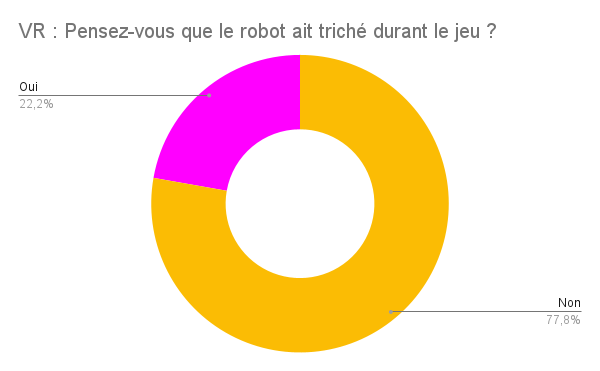
\includegraphics[width=\textwidth]{Datas/VR_triche.png}
    \captionof{figure}{VR}
    \end{minipage}%
    \vspace*{0.5cm}
    
    \subsubsection{How responsive did you find the robot to your answers?}
    \begin{figure}[!h]
    \centering
    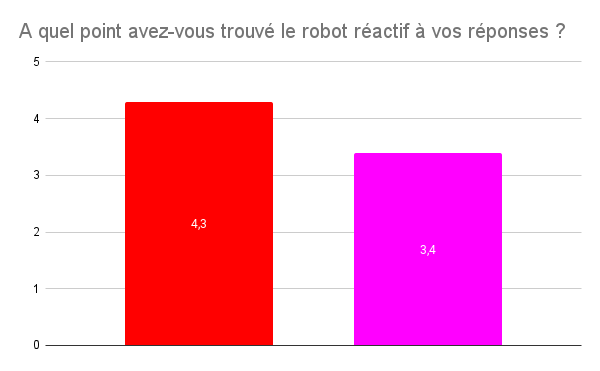
\includegraphics[height=4cm]{Datas/robot_react_reponse.png}
    \caption{Rouge : Physics, Magenta : VR}
    \end{figure}
    \vspace*{0.5cm}

    
    \subsubsection{Did this interaction feel natural to you?}
    \begin{figure}[!h]
    \centering
    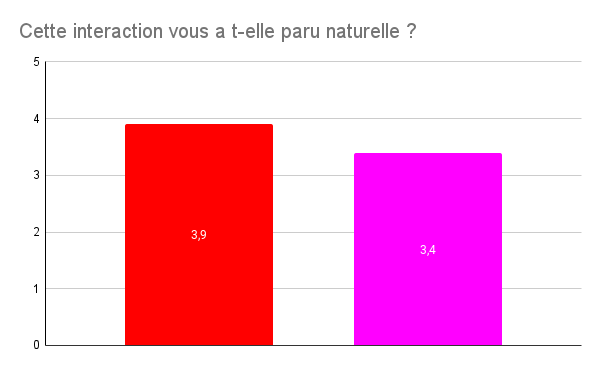
\includegraphics[height=4cm]{Datas/interaction_naturelle.png}
    \caption{Red : Physics, Magenta : VR}
    \end{figure}
    \vspace*{0.5cm}
    \newpage
    
    \subsubsection{How frustrating was the experience?}
    \begin{figure}[!h]
    \centering
    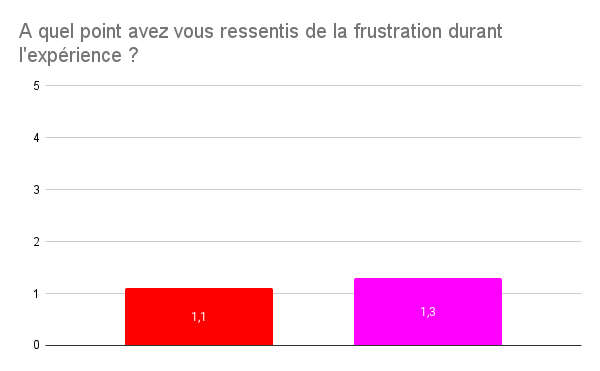
\includegraphics[height=4cm]{Datas/frustration.png}
    \caption{Red : Physics, Magenta : VR}
    \end{figure}
    \vspace*{0.5cm}

    \subsubsection{How did you feel interacting with the robot?}
    \begin{figure}[!h]
    \centering
    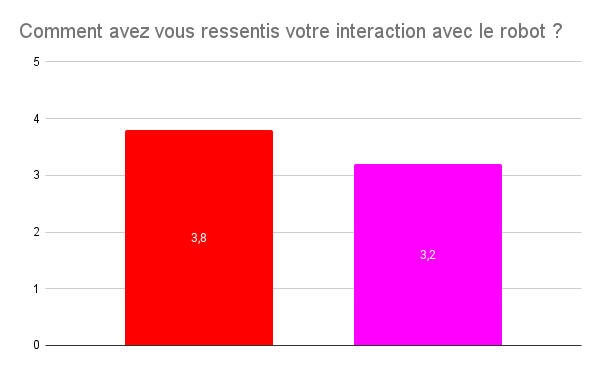
\includegraphics[height=4cm]{Datas/ressenti_interaction.png}
    \caption{Red : Physics, Magenta : VR}
    \end{figure}
    \vspace*{0.5cm}

    \subsubsection{Adult summary :}
Analysis of the data from our experiment revealed some interesting results regarding adults' perceptions of the robot, whether in its physical or VR version. Overall, they showed a relatively low level of empathy towards the robot, whatever its format \textit{(Figure 6.1 / Figure 6.2)}. They also considered that the physical robot possessed a slightly more distinct personality than the VR robot \textit{(Figure 6.3 / Figure 6.4)}.\\
Another notable point is that all the adults felt that the physical robot had not cheated, while some of them thought that the VR robot had adopted deceptive behaviors \textit{(Figure 6.5 / Figure 6.6)}. This divergence of opinion raises interesting questions about the perceived integrity and sincerity of virtual entities compared with those present in the physical world.\\
 They expressed positive impressions of the robots' responsiveness, and the interaction felt natural to them, whether in their physical or VR versions.\textit{(Figure 6.7 / Figure 6.8)} Participants also reported that they didn't feel much frustration throughout the experience \textit{(Figure 6.9)}. This suggests that the robots, whether physical or in VR, were able to provide tailored responses and feedback consistently.\\
\\

    \newpage
\subsection{Children}

    \subsubsection{Did the robot talk like a human?}
    \begin{minipage}{.5\textwidth}%
    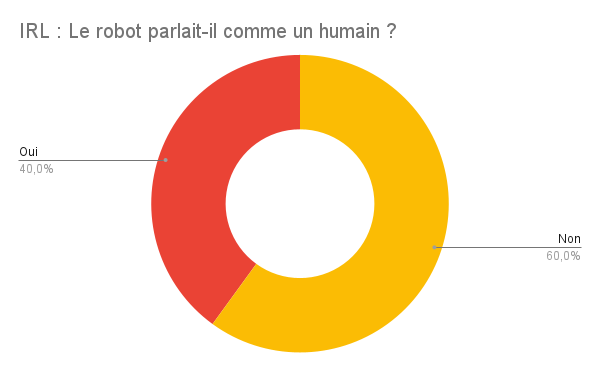
\includegraphics[width=\textwidth]{Datas_childs/IRL _ Le robot parlait-il comme un humain _.png}
    \captionof{figure}{Physics}
    \end{minipage}%
    \begin{minipage}{.5\textwidth}%
    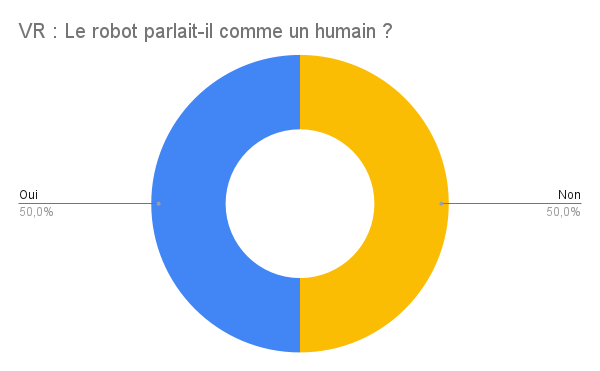
\includegraphics[width=\textwidth]{Datas_childs/VR _ Le robot parlait-il comme un humain _.png}
    \captionof{figure}{VR}
    \end{minipage}%
    \vspace*{0.5cm}

    \subsubsection{Did you feel any sympathy for the robot?}
    \begin{minipage}{.5\textwidth}%
    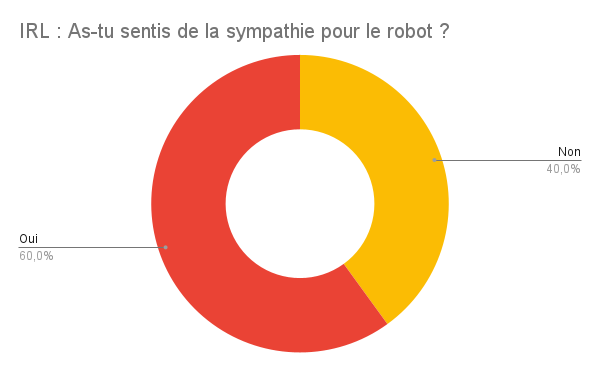
\includegraphics[width=\textwidth]{Datas_childs/IRL _ As-tu sentis de la sympathie pour le robot _.png}
    \captionof{figure}{Physics}
    \end{minipage}%
    \begin{minipage}{.5\textwidth}%
    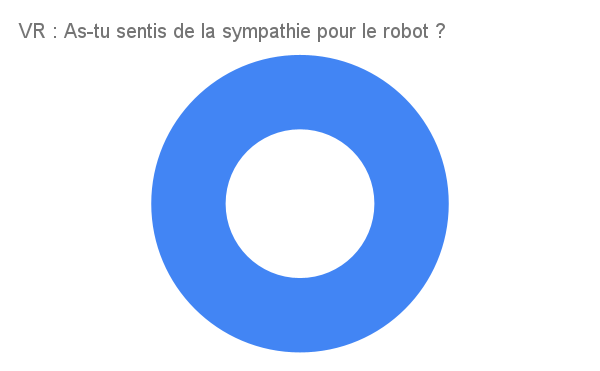
\includegraphics[width=\textwidth]{Datas_childs/VR _ As-tu sentis de la sympathie pour le robot _.png}
    \captionof{figure}{VR}
    \end{minipage}%
    \vspace*{0.5cm}

    \subsubsection{Do you think the robot cheated during the game?}
    \begin{minipage}{.5\textwidth}%
    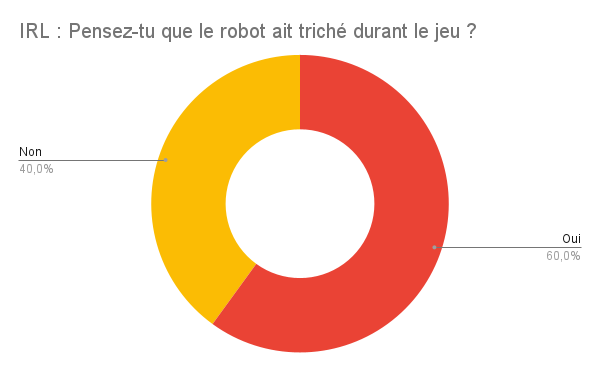
\includegraphics[width=\textwidth]{Datas_childs/IRL_triche_pendant_jeu.png}
    \captionof{figure}{Physics}
    \end{minipage}%
    \begin{minipage}{.5\textwidth}%
    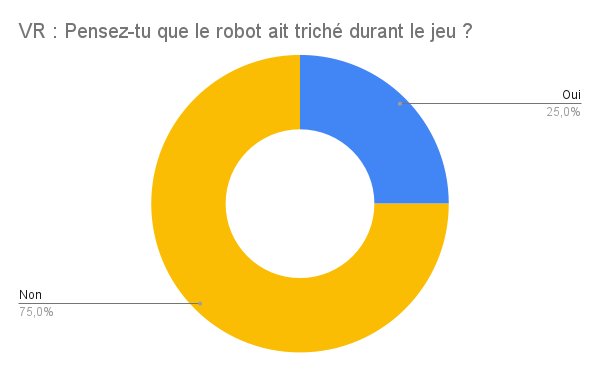
\includegraphics[width=\textwidth]{Datas_childs/VR_triche_pendant_jeu.png}
    \captionof{figure}{VR}
    \end{minipage}%
    \vspace*{0.5cm}
\newpage
    \subsubsection{Was it easy to talk to the robot?}
    \begin{figure}[!h]
    \centering
    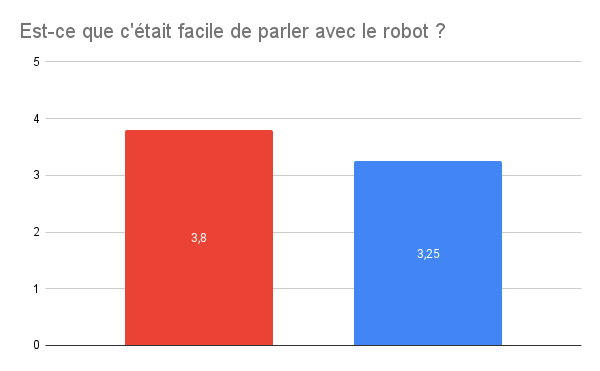
\includegraphics[height=5cm]{Datas_childs/facile_parler.png}
    \caption{Red : Physics, Magenta : VR}
    \end{figure}
    \vspace*{0.5cm}

    \subsubsection{Did the robot react quickly?}
    \begin{figure}[!h]
    \centering
    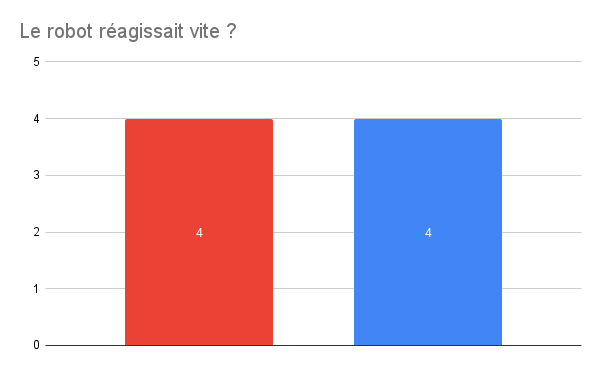
\includegraphics[height=5cm]{Datas_childs/reagit_vite_.png}
    \caption{Red : Physics, Magenta : VR}
    \end{figure}
    
    \vspace*{0.5cm}

    \subsubsection{Did you feel irritated?}
    \begin{figure}[!h]
    \centering
    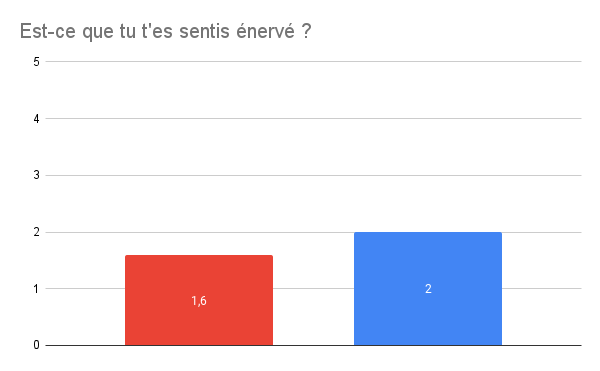
\includegraphics[height=5cm]{Datas_childs/enerve.png}
    \caption{Red : Physics, Magenta : VR}
    \end{figure}
    \vspace*{0.5cm}
    
    \vspace*{0.5cm}

    \subsubsection{Did you feel that the robot was nice or not?}
    \begin{figure}[!h]
    \centering
    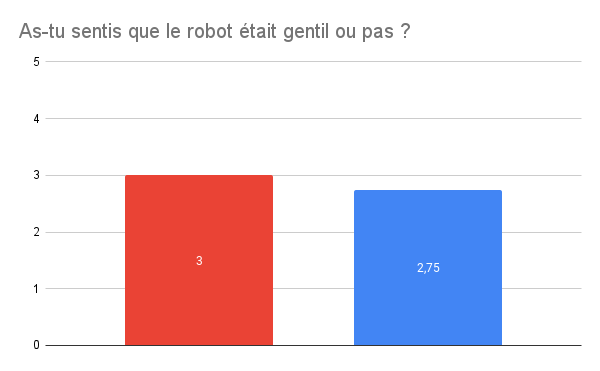
\includegraphics[height=5cm]{Datas_childs/gentil_ou_pas.png}
    \caption{Red : Physics, Magenta : VR}
    \end{figure}
    \vspace*{0.5cm}

\subsubsection{Children :}
During the children's participation in our experiment, interesting observations were made regarding their perception of the robot in virtual reality and in physics. The results show that half the children felt that the VR robot spoke like a human, with a slightly lower proportion for QTrobot \textit{(Figure 6.11 / Figure 6.12)}. It's also interesting to note that all the children felt sympathy towards the VR robot, while slightly more than half felt sympathy towards the physical robot \textit{(Figure 6.13 / Figure 6.14)}. This may suggest that the children were able to engage emotionally with the VR robot, perhaps due to its more abstract representation, whereas the tangible aspect of the physical robot elicited mixed reactions.\\
What's more, only a quarter of the children felt that the VR robot had cheated, while slightly more than half felt this way about the physical robot \textit{(Figure 6.15 / Figure 6.16)}. These results highlight a difference in perception of robot integrity between the two formats. It's possible that the children perceived the VR robot's actions as more controlled by algorithms or scripts, whereas the physical robot seemed to act more spontaneously and authentically.\\
The children found it rather easy to talk to the robot in virtual reality (VR), while it was slightly easier with the physical robot \textit{(Figure 6.17)}. The children also noted that the robots, whether in VR or physics, responded quickly \textit{(Figure 6.18)}. In terms of emotions, the children reported feeling slightly more irritated with the robot in VR, although overall they didn't feel much frustration during the experiment \textit{(Figure 6.19)}. On the other hand, the children gave a rather neutral response as to whether the robot was nice \textit{(Figure 6.20)}.
\newpage
\subsection{Overall summary :}
In conclusion, analysis of the data from our experiment highlights differences in perception and reaction between children and adults towards the robot in virtual reality (VR) and in physical reality. Children showed a greater propensity to perceive the VR robot as speaking like a human, to feel sympathy towards it and to find interaction easy. However, they were slightly more annoyed with the VR robot. On the other hand, adults showed relatively little empathy towards the robot, whether in VR or in physics. What's more, the adults felt that the physical robot had not cheated, while some thought that the VR robot had adopted deceptive behaviors.\\
\\
Both groups, children and adults, appreciated the robot's responsiveness, whether in VR or in physics, as well as the interaction, which was deemed natural. They reported little frustration throughout the experiment, suggesting that the robots were able to provide adapted responses consistently.\\
\\
It should also be noted that the data sample used in our analysis remains relatively small, with the participation of only 20 adults and 9 children. Due to the limited sample size, it is important to consider these results as preliminary observations rather than definitive generalizations. Further studies with larger and more diverse samples would be necessary to confirm and deepen our findings.\\
It's worth pointing out that had we had a larger data sample, we might have considered using machine learning models for further analysis to identify more complex patterns and relationships in the data, which could have provided additional insights into participants' responses, as well as more accurate predictions or classifications.\\

\chapter{Project management}
\section{SCRUM}
\subsection{The principle}
Project management is an essential element in guaranteeing the success of a project. For our project, we chose to adopt an approach based on agile methods, in particular the Scrum method. Agile methods are characterized by their flexibility, adaptability and iterative approach, making them particularly well suited to complex, evolving projects.\\
\\
The Scrum method is one of the most popular and widely used agile methods. Key Scrum practices include daily coordination meetings, during which each team member shares his or her progress, challenges and plans for the future. Sprint planning meetings are used to define the sprint objectives and select the features to be implemented. At the end of each sprint, a retrospective meeting is held to evaluate the previous sprint and identify improvements for future sprints.\\
\\
In our project, we implemented the method by organizing our team with specific roles: the Scrum Master and the development team.\\
\\
The Scrum Master is responsible for facilitating the Scrum process, removing obstacles and ensuring that the team follows Scrum principles and practices. He also ensures that the necessary meetings and interactions take place.\\
\\
The development team is responsible for completing project tasks and delivering functionality at the end of each iteration, called a "sprint". Sprints are short, intensive work cycles, generally lasting two to four weeks, during which the development team focuses on delivering the highest-priority features.\\
\\

\subsection{Adaptation for our project}
To adapt the Scrum method to our project, we made adjustments to meet our specific needs and constraints. The adaptations we made include:\\
\begin{enumerate}

\item \textbf{Sprint size and duration:} we started with one-week sprints accompanied by a weekly meeting. Then we adapted the duration of the sprints to the amount of work required.

\item \textbf{Team composition:} Ms Croitoru is our Scrum Master, and we make up the development team.
\item \textbf{Adapting meetings :} We have adjusted some Scrum rituals to better suit our needs. For example, during daily meetings, we have added a brief discussion of obstacles and specific problems encountered by the team, in order to resolve them more effectively.\\
\end{enumerate}
Using the Scrum method gave us a number of advantages, such as better visibility of project progress, rapid adaptation to changes and close collaboration between team members. Agile principles also fostered open and transparent communication, stimulating team commitment.\\

\begin{figure}[!h]
\centering
\includegraphics[height=10cm]{Figures/kanban.png}
\caption{Task kanban table - Notion}
\end{figure}

\newpage
\subsection{Distribution of tasks}
To optimize our efficiency, we chose to set up two-person mini-groups. This approach enabled us to take advantage of the complementary skills and knowledge of each team member, thus promoting greater productivity.
We thus set up two distinct groups, one dedicated to the development of the QTrobot and the other to virtual reality. Nevertheless, each person had the opportunity to work on both areas, which favored a thorough understanding of the project as a whole. \\
\\
Within each group, members worked in peer programming sessions. This method involves two developers working together on the same task, regularly exchanging ideas, solving problems together and ensuring the quality of the code produced. This enabled us to benefit from different points of view and find solutions more quickly.

\section{Tools used}
\subsection{Communication tools}
In addition to meetings with our supervisor at the IT building and at Lirmm, we used two essential communication tools: WhatsApp and Discord. These platforms played a key role in the coordination and collaboration between our team members.\\
\\
WhatsApp is an instant messaging application widely used around the world. We used it to facilitate fast, direct communication between the team and our project manager. WhatsApp's user-friendly interface and availability on smartphones make it a practical choice for instant communication.\\
\\
Discord, meanwhile, offers a host of features that foster online collaboration, such as chat rooms organized by category, voice channels for group calls and the ability to share files. We've used Discord for virtual meetings and group discussions, as well as for sharing important updates and resources. \\
\\
Using WhatsApp and Discord has greatly improved our efficiency and productivity as a team. These tools enabled seamless, instant and synchronized communication, promoting real-time collaboration. \\

\newpage
\subsection{Management tools}
We used two essential management tools to efficiently organize and manage our documents, information and tasks: Google Drive and Notion. We also used Overleaf to write the report in LaTeX.\\
\\
Google Drive is an online storage and file collaboration solution. We used it to create and share documents and photos. This platform enabled us to work simultaneously on the same files, promoting real-time collaboration. In particular, we used it to write and share roadmaps and meeting minutes, to keep a clear record of our progress. We also used the drive to share sound files, enabling us to implement voices for VR. \\
\\
Notion is a project management platform. We used it to organize our tasks, create checklists and track the progress of our various activities. The platform gave us an overview of all our tasks and deadlines, which helped us stay organized and meet our sprint deadlines. What's more, Notion allowed us to centralize all our important information in one place, facilitating sharing and collaboration between team members.\\
\chapter{Conclusion}

Despite these limitations and constraints, our team demonstrated adaptability and commitment to overcoming these obstacles. We implemented time management strategies, intensified our research, shared knowledge and worked autonomously when necessary. We also made strategic decisions to prioritize tasks and optimize our robot access time.\\
\\
It's also important to emphasize that our project differs from conventional programming projects. Our approach is based more on research and exploration of the psychological and behavioral aspects of human-robot interaction. This less conventional approach proved to be a wise choice, as it not only enabled us to acquire new knowledge and skills, but also piqued our interest in broader areas of computer science and robotics.\\
\\
It's worth pointing out that, despite the research orientation of our project, we still discovered many new technologies. We discovered what it was like to work with a real robot. We developed programming skills to set up the virtual reality experience and adapt the QTrobot's behavior. We also honed our modeling skills with the photogrammetry method. These complementary technical skills have enabled us to concretize our innovative research approach, combining theoretical and practical aspects for a better understanding of human-robot interaction.\\
\\
This multi-disciplinary approach has broadened our horizons and encouraged us to pursue our involvement in broader areas of computer science and robotics, where consideration of human factors is essential.\\
\\
In conclusion, our experience has demonstrated the importance of taking human and emotional aspects into account in the development of human-robot interactions. The results obtained and the knowledge acquired in the course of this project pave the way for new research and development perspectives in the field of human-robot interaction. We are proud to have taken part in this unique experiment, and are convinced that human-robot interaction will be at the heart of tomorrow's debates.
\chapter{Bibliography}

Robots Used In Therapy For Children With Autism Spectrum Disorder : \\
\url{https://www.ajmrd.com/wp-content/uploads/2022/03/E433339.pdf} \\

Social Humanoid Robots for Children with Autism Spectrum Disorders: A Review of Modalities, Indications, and Pitfalls : \\
\url{https://www.mdpi.com/2227-9067/9/7/953}\\

Towards metrics of Evaluation of Pepper robot as a Social Companion for Elderly People : \\
\url{https://www.uni-ulm.de/fileadmin/website_uni_ulm/iui.iwsds2017/papers/IWSDS2017_paper_24.pdf }\\

Emotion Recognition for Human-Robot Interaction: Recent Advances and Future Perspectives : \\
\url{https://www.frontiersin.org/articles/10.3389/frobt.2020.532279/full?utm_source=makeanapplike}\\

Emotion Recognizing by a Robotic Solution Initiative (EMOTIVE Project): \\
\url{https://www.mdpi.com/1424-8220/22/8/2861} \\

Revu de littérature :\\
\url{https://www.scribbr.fr/article-scientifique/revue-de-litterature-scientifique/} \\

Un atlas de l'interaction physique homme-robot tiré du livre Théorie des mécanismes et des machines: \\
\url{https://www.sciencedirect.com/science/article/abs/pii/S0094114X07000547#preview-section-references} \\

Le robot dans la clinique de l’autisme - Intérêts et enjeux futurs Par Olivier Duris\\
\url{https://www.techniques-ingenieur.fr/base-documentaire/innovation-th10/sciences-techniques-et-societe-42697210/le-robot-dans-la-clinique-de-l-autisme-ag119/}\\
ChatGPT :\\
\url{https://chat.openai.com/chat}\\
\newpage
J’étudie les relations homme-machine, vous m’avez posé vos questions par Fanny Chevalier : \\
\url{https://www.nouvelobs.com/rue89/rue89-posez-moi-vos-questions/20151008.RUE0844/j-etudie-les-relations-homme-machine-vous-m-avez-pose-vos-questions.html}\\

Interaction homme-robot par Hisour Art Cultur Histoire : \\
\url{https://www.hisour.com/fr/human-robot-interaction-42941/} \\

Documentation QTrobot :\\
\url{https://docs.luxai.com/}\\

Documentation Occulus with Unity :\\
\url{https://developer.oculus.com/documentation/unity}\\

Documentation LaTeX :\\
\url{https://www.xm1math.net/doculatex/mise_en_forme.html}

Notion: \\
\url{https://www.notion.so/}

\clearpage
\printglossary[type=\acronymtype]


\end{document}